\documentclass[a4paper, 15pt]{article}
\usepackage[left=0.85in, right=0.85in, top=0.5in, bottom=0.95in]{geometry}
\usepackage[T1]{fontenc}
\usepackage[utf8]{inputenc}
\usepackage[italian]{babel}
\usepackage[none]{hyphenat} % no sillabazione 
\usepackage{multicol} %testo su più colonne
\usepackage{enumerate}
\usepackage{enumitem}
\usepackage{mdwlist} %suspend enumerate \suspend{} \resume{}
\usepackage{lipsum} %testo random per verifica \lipsum
\usepackage{graphicx, nicefrac}
\usepackage{wrapfig2}
\usepackage{amsmath}
\usepackage{mathtools}
\usepackage{amssymb}
\usepackage{amsthm} %teoremi e dimostrazioni e definizioni
\usepackage{cases}
\usepackage{gensymb} %simboli come ° = \degree  etc etc
\usepackage{cancel} %permette di fare semplificazioni utilizzando il comando \cancel{expression}
\usepackage{subcaption}
\usepackage{hyperref}
\hypersetup{
	colorlinks=true,
	linkcolor=blue,    
	urlcolor=blue,
	%pdfpagemode=FullScreen, %il pdf generato non si avvia a schermo intero
}
\urlstyle{same}
\usepackage{changepage}
\usepackage{lastpage, epstopdf}
\usepackage{fancyhdr}
\usepackage{tcolorbox}
%\usepackage{background} %non utilizza lo sfondo con "draft"
\usepackage{color} % testo colorato \textcolor{'ColorCode'}{'testo'}
\usepackage{setspace} % in questo modo posso settare lo spoazio dell'indice \begin{spacing}{0.95}
	
\usepackage{changepage}
\usepackage{lastpage, epstopdf}
\usepackage{fancyhdr}
\usepackage{tcolorbox}
%\usepackage{background}
\usepackage{tikz} %disegni e mappe
\usetikzlibrary{patterns}
\usepackage{pgfplots}
\pgfplotsset{compat=1.15}
\usepackage{mathrsfs}
\usetikzlibrary{arrows,decorations.markings}
\raggedbottom
\setlength{\parindent}{0pt}
%%%%%%%%%%%%%%%%%%%%%%%%%%%%%%%%%%%%%%%%%%%% SIUNITX 
\usepackage{siunitx}

%========TEOREMI========%
\newtheorem*{thm}{Teorema}
\newtheorem*{en}{Enunciato}
\newtheorem*{definizione}{Definizione}
\newtheorem*{cor}{Corollario}



%========OPERATORI&COMANDI========%
\DeclareMathOperator{\rk}{rk}
\DeclareMathOperator{\im}{Im}
\DeclareUnicodeCharacter{20AC}{\EUR}
\newcommand{\cmark}{\ding{51}}
\newcommand{\xmark}{\ding{55}}
\newcommand{\compresslist}{ % Define a command to reduce spacing within itemize/enumerate environments, this is used right after \begin{itemize} or \begin{enumerate}
			\setlength{\itemsep}{1pt}
			\setlength{\parskip}{0pt}
			\setlength{\parsep}{0pt}
		}
		\newcommand{\ra}[1]{\renewcommand{\arraystretch}{#1}} %stretcho le tabelle
		
		%\renewcommand{\arraystretch}{2.5} % Da copiaincollare prima di ambienti array per ampliarli un po'
		%\setlength{\jot}{10pt} % affecting the line spacing in the environment SPLIT
	
\begin{document}
		\setcounterpageref{secnumdepth}{0}	
		\tableofcontents 
		\newpage
	
\part{1. METROLOGIA}	
\section{Introduzione}	
	\begin{adjustwidth}{2in}{}
		Treccani: La metrologia è la scienza della misura, ovvero la disciplina che si occupa di
	definire le procedure per eseguire corrette misurazioni. 
	
	In che senso corrette? Come si ottiene una \underline{corretta} misurazione? È quella la parte complicata, è necessario minimizzare l'errore, l'incertezza.
	
	La metrologia si basa su analisi sperimentali, questo strumento garantisce da una parte la qualità del prodotto, ma dall'altra può incedere pesantemente sul costo di tale prodotto.
	
	Chiunque effettua analisi sperimentali incorre nel rischio di non avere metodi riconosciuti e quindi di incappare in risultati incerti e questo si aggrava se le procedure di misura non si riferiscono a campioni univoci. 
	
	Tali analisi sperimentali aprono così le porte alle finalità delle misure, che fine ha ciò che misuro? \newline
	

		\begin{itemize}
 		\item \textbf{Metrologia legale}
		
		Studia unità di misura, metodi e strumenti in modo da garantire la correttezza delle misure utilizzate nelle transazioni commerciali;
		
		\item \textbf{Metrologia scientifica} 
		
		Ha come obiettivo la determinazione di modelli fisici (fini di ricerca);
		
		 \textbf{Metrologia industriale} 		
		\begin{enumerate}
			\item Verifica di conformità dei prodotti realizzati rispetto ai requisiti specificati (valore di tolleranze, ecc); 
			\item Controllo del processo produttivo (la verifica del prodotto finale non garantisce l’assenza di anomalie che potrebbero determinare lo scarto del prodotto).
		\end{enumerate}
		\end{itemize}
	\end{adjustwidth}		


\subsection{Documenti di riferimento} 
	\begin{adjustwidth}{2in}{}
	\textbf{VIM} 
	
	“International vocabulary of basic and general terms in metrology”, edito
	dalla ISO nel 1984 ed aggiornato nel 1987, nel 1993, nel 2008 e nel 2012. \newline
	
	Il VIM è internazionalmente usato e riconosciuto, queste sono altre norme per cultura generale:
	\begin{itemize}
		\item UNI 4546 "Misure e misurazioni - Termini e definizioni fondamentali” 1984; 
		\item UNI EN ISO 8402 "Gestione per la qualità ed assicurazione della qualità.
		Termini e definizioni 1995;
		\item UNI EN 30012 Parte 1 "Requisiti di assicurazione della qualità relativi agli
		apparecchi per misurazioni. Sistema di conferma metrologica di apparecchi
		per misurazioni" 1994
	\end{itemize}
	\end{adjustwidth}
\newpage 

\subsection{Misurazione} 	
	\begin{adjustwidth}{2in}{}
		La misurazione è la determinazione del valore numerico di una grandezza fisica per mezzo del rilievo dell'output di una catena di misura. 
	
	I passi che si effettuano nell'azione di misurazione prevedono un punto di partenza, ovvero la realtà tangibile, che attraverso un modello viene misurata, ed è esattamente questo il concetto da trasmettere, è il modello che si misura, è necessario perciò formalizzare e caratterizzare tale modello secondo opportune relazioni tra grandezze e solo dopo, in dipendenza del tipo di misura necessaria, si potrà scegliere lo strumento più adeguato alla misura. 
	
	È il modello ad essere scelto in funzione dello scopo delle misure da effettuare, tenendo bene a mente però che: 
	\begin{itemize}
		\item Un modello non ha mai validità assoluta;
		\item Non è necessario complicare a tutti i costi il modello;
		\item È necessario valutare economicamente della complessità del modello;
	\end{itemize}
	Il classico esempio può essere la misura dell'area di un rettangolo dai lati frastagliati, si può considerare sia il triangolo regolarmente costruito circoscritto all'oggetto della misurazione; oppure un rettangolo inscritto al quale si sommeranno aree di piccoli triangoli e rettangoli ottenuti riempiendo le zone rimaste scoperte.	
	\end{adjustwidth}
\subsection{Alcune definizioni} 		
	\begin{adjustwidth}{2in}{}
		\begin{itemize}
		\item \textbf{Misurando}: grandezza che viene sottoposta a misurazione;
		\item \textbf{Grandezza Estensiva}: dipende dalla dimensione del corpo, Vale l’operazione somma, si ottiene per confronto eseguito in termini di rapporti;
		\item \textbf{Grandezza Intensiva}: non dipendente dalle dimensioni del corpo, non vale l'operazione di somma, rapporti legati unicamente a differenze rispetto ad un valore di riferimento.
		\item \textbf{Misura diretta}: Si ottiene per confronto diretto con l'unità di misura ed i suoi multipli o sottomultipli, per cui non è necessario conoscere esplicitamente nessuna altra grandezza al di fuori di quella letta dallo strumento di misura;
		\item \textbf{Misura indiretta}: Si ottiene mediante l'applicazione di leggi fisiche che legano la grandezza incognita ad altre misurabili direttamente, per cui si perviene al risultato mediante relazioni di calcolo che presuppongono una
		misura diretta di due o più parametri.
	\end{itemize}
	
\textbf{Misura} 

	La misura è un'informazione formata da un numero, un incertezza ed una unità di misura:
	\[ X= (x \pm u)g \]
	Un valore così definito non si pone essere l'unica verità ma rappresenta l'intervallo di valori tra i quali è compreso il vero valore. 
	
	L'incertezza così definita sarà dipendente non sono dallo strumento in termini di qualità e risoluzione, ma anche dall'operatore e dall'ambiente. 
	
\textbf{Compatibilità delle misure} 

	Due misure dello stesso misurando condotte da differenti operatori con
	differenti strumenti e metodologie, e in diversi tempi e luoghi, non devono
	risultare necessariamente uguali, ma devono essere comunque compatibili.
	
	Due misure sono compatibili quando presentano almeno un elemento della
	fascia di valori x ± u in comune.
	
\begin{figure}[H]
	\centering
	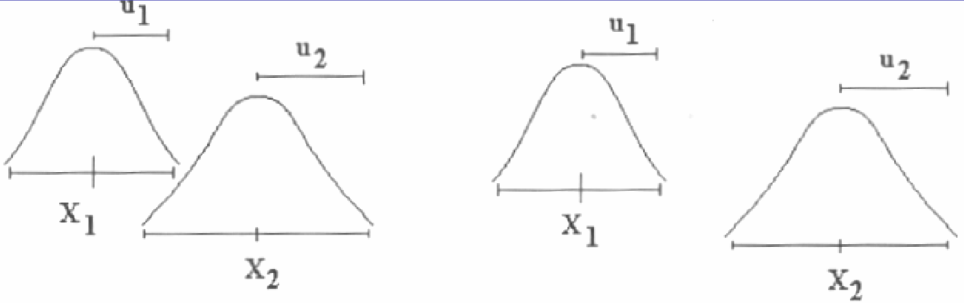
\includegraphics[width=0.5\linewidth]{fig/screenshot001}
	\label{fig:screenshot001}
\end{figure}
\end{adjustwidth}

\newpage
\subsection{Regole di scrittura} 
\begin{adjustwidth}{2in}{}
	\begin{itemize}
		\item Utilizzo di un punto a mezz'altezza o di uno spazio per indicare unità derivate
		ottenute dal prodotto di altre unità (N·m o N m);
		\item Utilizzo di una barra obliqua, orizzontale o di esponenti negativi per indicare
		unità derivate ottenute dal rapporto di altre unità (es. m/s o m·s-1);
		\item Utilizzo delle forme esponenziali per indicare unità derivate ottenute dal
		rapporto o dal prodotto di altre unità ogni volta che possano generarsi
		ambiguità;
		\item Non si deve far seguire sulla stessa linea dopo una barra obliqua un segno di
		moltiplicazione o di divisione;
		\item Utilizzo di uno spazio tra numero e unità;
		\item Non inserire alcuno spazio tra prefisso e simbolo della unità;
		\item Non usare simboli composti di più prefissi;
		\item Il simbolo dell’unità non va seguito dal punto;
		\item Scrittura per esteso dei prefissi e dei simboli, quando questi non sono
		accompagnati da valore numerico;
		\item Utilizzo dell'iniziale minuscola per le unità caratterizzate da un nome proprio
		(es. joule, watt, ecc.), ma dell'iniziale maiuscola in presenza di simbolo (es. J,
		W, ecc.);
		\item I valori di misura devono essere espressi utilizzando multipli e sottomultipli
		delle unità di misura, così da riportare i valori numerici nel campo compreso
		tra 0,1 e 999;
		\item Uso del plurale per le sole unità SI: metro, secondo, ecc;
		\item I simboli di ora, minuto e secondo sono h, min, s (non hr, ’, ’’).
	\end{itemize}
\end{adjustwidth}

\section{Sistema di unità di misura}
\begin{adjustwidth}{2in}{}
	Ci si è trovati con la necessità di definire un numero di grandezze fisiche indipendenti e fondamentali dalle quali derivino grandezze derivate. 
	
	È stato perciò necessario adottare un sistema di unità di misura al quale dover collegare una serie di campioni con lo scopo di unificare le misurazioni. 
	
	Così per ogni branca della fisica è stato necessario definire:
	\begin{itemize}
		\item lunghezza per la geometria;
		\item tempo per l'astronomia;
		\item la massa e la forza  per la dinamica;
		\item la temperatura per la termodinamica;
		\item la corrente per l'elettromagnetismo (passando dalla carica elementare e la resistenza);
		\item l'intensità luminosa per l'ottica;
		\item la mole per la quantità di sostanza..
	\end{itemize}

	Un sistema di unità di misura deve perciò rispondere ai seguenti requisiti: 
	\begin{itemize}
		\item \textbf{omogeneità}: dalle grandezze fondamentali possono essere derivate tutte le altre grandezze;
		\item \textbf{assolutezza}: il campione deve essere scelto sulla base di leggi universali della fisica, non deve dipendere dai materiali impiegati;
		\item \textbf{universalità}: il campione deve essere accettato da tutti;
		\item \textbf{riproducibilità}: il campione deve poter essere realizzato in luoghi e tempi diversi senza presentare differenze significative;
		\item \textbf{stabilità}: i campioni del sistema di misura devono essere stabili, ovvero connessi a fenomeni o grandezze fisiche inalterabili nel tempo;
		\item \textbf{praticità}: le grandezze fondamentali devono avere un senso fisico immediato e non creare problemi pratici di apprendimento e uso;
		\item coerenza: una qualsiasi unità deve poter essere espressa mediante un legame del
		tipo:
		\[g = m^a kg^b s^g A^d K^e cd^q mol^f\]
		In cui  coefficienti $a,b,…,f$ possono assumere il valore di zero o di un numero intero,	positivo o negativo.
		\item \textbf{indipendenza} delle grandezze fondamentali: il sistema di misura deve essere costituito da un numero k di grandezze fondamentali indipendenti, le restanti
		grandezze devono poter essere derivate sulla base delle relazioni fisiche o
		geometriche esistenti tra tali grandezze;
		\item \textbf{uniformità}: le scale di misura di ciascuna grandezza devono essere uniformi, deve essere possibile ricavare il valore di un qualunque intervallo mediante due letture lungo la scala.
	\end{itemize}
\end{adjustwidth}

\subsection{Definizioni}
\begin{adjustwidth}{2in}{}
	Il primo sistema di unità di misura nacque dalla necessità di definire univocamente l'elettromagnetismo: Sistema mksA. 
	
	Cambiano il riferimento in sottomultipli di quello considerato si ottiene il Sistema cgs, dove le sole unità di misura utilizzate divengono il centimetro per la lunghezza, il grammo per la massa e il secondo per il tempo, in questo modo di ottengono: 
	\begin{itemize}
		\item velocità $[cm/s]$
		\item Accelerazione $[cm/s^2]$
		\item Forza [dine]: forza che applicata ad un corpo di massa 1 g gli conferisce una accelerazione pari
		a 1 $[cm/s^2]$
		\item Lavoro [erg]: lavoro compiuto da una forza di 1 dine per spostare un corpo di 1 cm
		\item Energia [caloria, cal]: quantità di calore che si deve fornire alla massa di 1 g di acqua distillata per portare la
		sua temperatura da 14,5 $\degree$ C a 15,5 $\degree$ C.
		
		Notare come la caloria ed i suo multiplo kilocaloria (che fa riferimento ad 1 kg di acqua) vengano usati tuttora oggi.
	\end{itemize}

	Un sistema di seguito introdotto per tentare di perseguire una certa uniformità è il sistema tecnico, come per il sistema cgs si definiscono le grandezze fondamentali e da quelle si ricavano le derivate. 
	
	Se per la lunghezza si utilizza il metro, per la forza il kilogrammo forza e per il tempo il secondo si ottengono: 
	\begin{itemize}
	\item $kg_f$ 	è una la grandezza fondamentale ed è definita come il peso (la forza peso) di una massa di
	1 kg in condizioni di gravità campione (9,80665 $m/s^2$);
	\item L’unità di massa è un'unità derivata e prende il nome di “unità di massa
	pratica”, questa è definita come quella massa che, sottoposta ad una
	forza pari a 1 $kg_f$, accelera di 1 $m/s^2$.
	\[ 1m_p = \dfrac{1kg_f}{1m/s^2} \]	 
	\end{itemize}

	Si possono operare, a questo punto, le conversioni tra il sistema tecnico e il sistema internazionale. 
	\[ 1kg_f = 1kg \cdot 9,80665 m/s^2 = 9,80665N \approx 10N \]
	\[ 1m_p = \dfrac{1kg_f}{1m/s^2} = \dfrac{1kg \cdot 9,80665 m/s^2}{1m/s^2} = 9,80665kg \approx 10kg \]
	Quanto pesa (inteso come forza peso) l'unità di massa pratica?
	\[1m_p \cdot 9,80665 m/s^2 = \dfrac{1kg_f}{1m/s^2} \cdot 9,80665 m/s^2 = 9,80665kg_f \approx 10kg_f \]
	Notare come il numero che esprime la massa nel SI (kg) è lo stesso che esprime il peso nel sistema tecnico/pratico, dove il pedice "f" è stati aggiunto per semplicità di identificazione. 
	
	Inoltre, va notato che normalmente nel parlato, quando si fa riferimento al peso di un qualcosa, oggetto o persona, lo chiamiamo peso, e non forza peso, utilizzano implicitamente e inconsapevolmente il sistema tecnico. 
	
	Nel sistema tecnico l'unità di lavoro e di energia è il kilogrammetro $kg_fm$, che corrisponde a:
	\[ 1kg_f\cdot m \approx 10N\cdot m = 10J\]
	L'unità di potenza è il $kg_fm/s$ di cui si definisce il multiplo chiamato cavallo vapore CV ancora largamente utilizzato oggi, tale cavallo vapore è definito come $75kg_fm/s$, a quanti watt corrisponde?
	\[ 1kg_fm/s \approx 10J/s = 10W \Rightarrow 75kg_fm/s = 750W  \]
	
	Similmente al sistema cgs si introduce il sistema di misura britannico fps, basato questo sul piede (foot) per la misura della lunghezza, la libbra (poud) per la misura della massa e il secondo per la misura del tempo, in cui:
	
	\[ 1ft = 30.48cm\]
	\[ 1lb = 453.6g\]
	
	L'unità di forza è il poundal (pdl) definito come quella forza che imprime alla massa di 1lb l'accelerazione di 1$ft/s^2$. 
	
	L'unità di energia è il foot poundal. \newline
	
	in maniera simile al sistema tecnico il sistema britannico flbs utilizza il piede (foot) per la misure delle lunghezze, la libbra forza (foot poundal) per la misura della forza e il secondo perla misura del tempo. 
	\begin{itemize}
		\item la libbra forza $lb_f$ è una grandezza fondamentale ed è definita come il peso di
		una massa di 1lb in condizioni di gravità campione 32,17 $ft/s^2$;
		\item L’unità di massa è una unità derivata e prende il nome di “slug”, questo è definito come quella massa che, sottoposta ad una forza pari a 1$lb_f$,
		accelera di 1$ft/s^2$.
		
		Come per il sistema tecnico si possono identificare delle conversioni:
		\[ 1lb_f = 1lb \cdot 32.17 ft/s^2 = 32.17 pdl \]
		\[ 1slug = \dfrac{1lb_f}{1ft/s^2} = \dfrac{1lb \cdot 32.17 ft/s^2}{1ft/s^2} = 32.17 lb \]
		Quanto pesa uno slug?
		\[ 1slug \cdot 32.17 ft/s^2 = \dfrac{1lb_f}{1ft/s^2} \cdot 32.17 ft/s^2 = 32.17 lb_f  \]
	\end{itemize}

	A partire così dal sistema mksA si arriva finalmente al Sistema Internazionale SI aggiungendo le misure di temperatura, intensità luminosa e quantità di sostanza.

	Alle quali si possono aggiungere due grandezze supplementari: il radiante per misurare un angolo piano e lo steradiante per misurare l'angolo solido. 
	
	\begin{itemize}
		\item \textbf{Intervallo di tempo} 
		 
		Il secondo è la durata di 1'192'631'770 periodi della radiazione corrispondente alla transizione fra i due livelli iperfini dello stato fondamentale dell'atomo di cesio 113. 
		
		Non è poi così pratica...
		
		\item \textbf{Lunghezza} 
		
		Il metro è la lunghezza del tragitto percorso dalla luce nel vuoto in un intervallo di 1/299'792'458 di secondo.
		
		Essendo la velocità di propagazione della luce nel vuoto una costante fondamentale della fisica, con questa definizione il valore assunto dal metro è esatto, privo di incertezza e immodificabile. 
		
		\item \textbf{Massa} 
		
		Il kilogrammo è l'unità di massa, esso è pari alla massa del prototipo internazionale del kilogrammo. 
		
		Questa definizione manca di assolutezza...  
		
		Il kilogrammo prototipo è stato definito e copiato e le copie distribuite. Ora, tali copie non saranno mai esenti da difetti di fabbricazione e produzione, pertanto avranno insite incertezze sul rispettivo peso, cosa succede se si usano copie anche minimamente incerte per ottenere una scala di misurazione a partire dal prototipo? Che le incertezze si propagano e possono arrivare anche a 40mg sul grammo, e come se non bastasse, per tenere traccia della veridicità del campione lungo gli anni, è stata tenuta traccia della variazione del suo peso, con risultati non piacevoli.

		Ha senso effettuare la misura se il suo campione varia? 
		
		\item \textbf{Temperatura} 
		
		Il kelvin, unità di misura termodinamica, è la frazione 1/273.16 della temperatura termodinamica del punto triplo dell'acqua. 
		
		Questa è una misura che manca di assolutezza e di indipendenza, si affida dapprima ad un materiale, l'acqua, sapendo che la temperatura della stessa può variare con la pressione.
		
		\item \textbf{Quantità di sostanza }
		
		La mole è la quantità di sostanza di un sistema che contiene tante entità elementari quanti sono gli atomi in 0.012kg di carbonio 12. Quando si usa la mole le quantità elementari devono essere specificate; esse possono essere atomi, molecole, ioni, elettroni, altre parcticelle oppure raggruppamenti specificati di tali particelle. \newline
		
		Questa è una definizione che manca di indipendenza. 
		
		\item \textbf{Intensità di corrente elettrica} 
		
		L'ampere è l'intensità di una corrente elettrica costante che, mantenuta in due conduttori paralleli rettilinei di lunghezza infinita, di sezione circolare trascurabile, posti alla distanza di un metro l'uno dall'altro nel vuoto, produrrebbe tra questi conduttori una forma eguale a $2\times10^{-7}$ newton su ogni metro di lunghezza. \newline
		
		È una definizione che pecca di indipendenza, in più è fondata su di un esperimento ideale.
		
		\item \textbf{Intensità luminosa} 
		
		La candela è l'intensità luminosa, in una determinata direzione, di una sorgente che emette una radiazione monocromatica di frequenza $540\times10^{12}$ hertz e la cui intensità energetica in tale direzione è 1/683 watt allo steradiante. 
		
		Anche qua si pecca di indipendenza. 
	\end{itemize}
\newpage
	Valido dal 20 maggio 2019 è stato introdotto un nuovo sistema internazionale in cui non sussisterà più la divisione tra grandezze fondamentali e derivate, ma saranno tutte  derivate a partire da costanti fisiche universali, per cui ciò che cambieranno saranno soltanto le definizioni.
	
	In questo modo si garantisce la riproducibilità delle misure e la totale assenza di incertezza dovuta alla realizzazione del campione.
	
\begin{figure}[H]
	\centering
	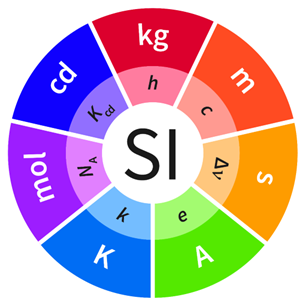
\includegraphics[width=0.5\linewidth]{fig/screenshot002}
	\label{fig:screenshot002}
\end{figure}


	\begin{itemize}
		\item \textbf{Secondo} 
		
		Il secondo, il cui simbolo è s, è l'unità di misura di base del tempo; è definito dal valore numerico della frequenza della transizione iperfine $(\Delta\nu_{Cs})$ dello stato fondamentale imperturbato dell'atomo di cesio 133, fissato a 9 192 631 770 quando espresso nell'unità di misura Hz, che equivale a $s^{-1}$.
		\[ \Delta\nu_{Cs} = 9 192 631 770 Hz \]
		\[ 1 Hz = \dfrac{\Delta\nu_{Cs}}{9 192 631 770} \Rightarrow 1 s = \dfrac{9 192 631 770}{\Delta\nu_{Cs}} \]
		Tale definizione coincide tra l'altro con la precedente definizione di secondo.
		
		\item \textbf{Metro} 
		
		Il metro, il cui simbolo è m, è l'unità di misura di base della lunghezza; è definito dal valore numerico della velocità della luce nel vuoto (c) fissato a 299 792 458 quando espresso nell'unità di misura m/s, dove il secondo è definito in termini di $(\Delta\nu_{Cs})$. 
		\[1m = \left( \dfrac{c}{299 792 458}\right)s = \dfrac{ 9 192 631 770}{299 792 458}\dfrac{c}{\Delta\nu_{Cs}} \]
		Anche in questo caso, affermando che il metro è la lunghezza del percorso compiuto dal raggio di luce nel vuoto in un intervallo di tempo pari a 1/299 792 458, rimanda alla vecchia definizione di metro.
		
		\item \textbf{Chilogrammo} 
		 
		Il chilogrammo o kilogrammo, il cui simbolo è kg, è l’unità di misura di base della massa.
		
		È definito a partire dal valore numerico fisso della costante di Planck (h), pari a 6.626 070 15 $\times10^{-34}$  quando espressa nell'unità J s, che corrisponde a kg $m^2 s^{-1}$, dove il metro e il secondo sono definiti a partire da c e $\Delta\nu_{Cs}$.
		\[ 1kg = 1.475 521 4 \times 10^{40} \dfrac{\Delta\nu_{Cs}h}{c^2}\]
		
		\item \textbf{Ampere} 
		
		L'ampere, il cui simbolo è A, è l'unità di misura di base dell'intensità di corrente elettrica; è definito dal valore numerico della carica elementare (e) fissato a 1,602 176 634 $\times 10^{-19}$ quando espressa nell'unità di misura C, che equivale a A s, dove il secondo è definito in termini di $\Delta\nu_{Cs}$. 
		\[ 1 A \approx 6.789 687 \times 10^8 \Delta\nu_{Cs}e\]
		
		\item \textbf{Kelvin} 
		
		Il kelvin, il cui simbolo è K, è l’unità di misura di base della temperatura termodinamica; è definito fissando il valore numerico della costante di Boltzmann (k) a 1.380 649 $\times 10^{-23}$ quando espresso nell’unità J $K^{-1}$, che è equivalente a kg m2 $s^{-2} K^{-1}$, dove il chilogrammo, il metro e il secondo sono definiti in termini di h, c e $\Delta\nu_{Cs}$.
		
		\[ 1K = 1.266 665 3 \dfrac{\Delta\nu_{Cs}h}{k}\]
		
		\item \textbf{Mole} 
		
		La mole, il cui simbolo è mol, è l’unità di misura di base della quantità di sostanza; una mole contiene esattamente 6,022 140 76 $\times 10^{23}$ entità elementari; tale numero è il valore fissato per la costante di Avogadro NA, quando espressa nell’unità mol$^{-1}$, ed è detto numero di Avogadro; la quantità di sostanza (n) di un sistema è la misura del numero di specifiche entità elementari. Un’entità elementare può essere un atomo, una molecola, uno ione, un elettrone, ogni altra particella o gruppi di particelle.
		
		\[ 1mol = \left( \dfrac{6.022 140 76 \times 10^{23}}{N_A} \right) \]
		
		\item \textbf{Candela} 
		
		La candela, il cui simbolo è cd, è l'unità di misura di base dell'intensità luminosa in una data direzione; è definita dal valore numerico prefissato del coefficiente di visibilità della radiazione monocromatica con frequenza 540 x 1012 Hz, $K_{cd}$, pari a 683, espresso in lm $W^{-1}$, o in cd sr $W^{-1}$ (che equivale a cd sr $kg^{-1}$ $m^{-2}$ $s^3$), dove il kilogrammo, il metro e il secondo sono definiti in termini di h, c  e $\Delta\nu_{Cs}$.		
	\end{itemize}
	
	Con il nuovo sistema internazionale gli istituti metrologici possono scegliere l'equazione fisica per "costruire" il campione dell'unità di misura a partire da costanti note e misurabili, inoltre si perde il problema dell’incertezza legata alla definizione del campione dell’unità di misura, senza contare che in futuro si potranno trovare diversi modi di realizzare l’unità di misura a partire dalle costanti senza dover cambiare il sistema di riferimento. 
	
\begin{figure}[H]
	\centering
	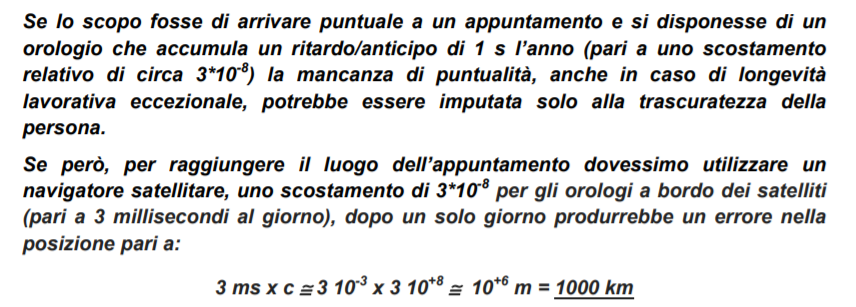
\includegraphics[width=0.5\linewidth]{fig/screenshot003}
	\label{fig:screenshot003}
\end{figure}
\end{adjustwidth}
\newpage
\subsection{Unità di misura} 
\begin{adjustwidth}{2in}{}
	La misura di una grandezza fisica A è possibile quando è nota una grandezza
	U omogenea con A:
	\[x = \dfrac{A}{U}\]
	In questo modo la grandezza A è pari ad x volte la grandezza U, dove U prende la forma di una grandezza campione o unità.
	
	Esempio: Misurare la lunghezza della scrivania con il metro
	
	La lunghezza (A) è 1,5 (x) volte il metro “campione” (U)
	
\subsection{Fattore di ragguaglio} 
	Si consideri una nuova unità U' con cui si esprime la misura di A: 
	\[ x' = \dfrac{A}{U'} \ne x\]
	Identifico U' come nuova unità di misura per cui la grandezza A è pari a x' volte la grandezza U' e in cui, per passare da x a x' basta scrivere:
	\[\dfrac{A}{U'} = \dfrac{A}{U} \dfrac{U}{U'} = \dfrac{A}{U} \cdot \tau \]
	In cui\[ \tau= \dfrac{U}{U'} \dfrac{\text{unità di misura precedente/di partenza}}{\text{nuova unità di misura/di arrivo}}\]  prende il nome di fattore di ragguaglio. 
	\[ \text{unità di partenza} ~ = \tau ~ \text{unità di arrivo}\]\newline
	\textbf{NB}: IL RAPPORTO DEV'ESSERE OMOGENEO. \newline
\end{adjustwidth}
\newpage	
\subsubsection{Esercizi sul fattore di ragguaglio} 

	Da mm a km
	\[\tau = \dfrac{U}{U'} = \dfrac{1mm}{1km} = \dfrac{1mm}{10^6mm}= 10^{-6}\]
	Da secondi ad ore
	\[\tau = \dfrac{U}{U'} = \dfrac{1s}{1h} = \dfrac{1s}{3600s}= 1/3600\]
	
	
\textit{\textbf{Grandezze fondamentali e  derivate}} 
	\begin{itemize}
		\item Lunghezza [L] grandezza fondamentale;
		\item Area grandezza derivata [A] = [L$\times$L];
		\item Volume grandezza derivata [V] = [L$\times$L$\times$L]
	\end{itemize}
	In un rettangolo le dimensioni sono a=[cm]=b, qual è l'area espressa in millimetri? Ci si chiede quindi dapprima a quanti mm equivalgono le misure in cm (cm = $\tau_{mm} \cdot$ mm) e poi si effettua l'operazione considerando il fattore di ragguaglio. 
	\[A = a\cdot b =\tau_a mm \cdot \tau_b mm =ab (cm/mm)^2 mm^2 = \tau^2 mm^2 \]
	
	\textbf{\textit{Grandezze cinematiche, da 3m/s a cm/h}} 
	\[ \begin{dcases}
		\tau_{cm} = \dfrac{1m}{1cm} = \dfrac{100cm}{1cm} = 100 \\
		\tau_h = \dfrac{1s}{1h} = \dfrac{1s}{3600s} = 1/3600
	\end{dcases} \Rightarrow \tau_{cm/h} = \dfrac{\tau_{cm}}{\tau_h} = \dfrac{100}{1/3600} = 360'000 \]
	La nuova velocità sarà pari a:
	\[ 3m/s = 3 \cdot \tau_{cm/h} \cdot cm/h = 1'080'000 cm/h \]
	
	 \textbf{\textit{Grandezze dinamiche, da 3N a dine}} 
	 \[ N = \dfrac{kg\cdot m}{s^2} \rightarrow dine = \dfrac{g\cdot cm}{s^2} \]
	\[ \begin{dcases}
		\tau_g = \dfrac{1kg}{1g} = \dfrac{1000g}{1g} = 1000 \\
		\tau_{cm} = \dfrac{1m}{1cm} = \dfrac{100cm}{1cm} = 100 \\
		\tau_s = 1
	\end{dcases} \Rightarrow \tau_{dine} = \dfrac{\tau_g\tau_{cm}}{\tau_s} = 10^5 \]
	E dunque avremo:
	\[ 3N = 3\tau_{dine} \cdot dine= 3\cdot 10^5 dine\]
	
	\textit{\textbf{Pressione, da mmHg a Pa}}  
	\[ mmHg = \dfrac{1}{760} atm\]
	\[ atm = ~ \text{pressione di una colonna di mercurio di 760mm} ~ = \rho g h\]
	\[\rho_{Hg} = 13'595 kg/m^3 \Rightarrow atm = 13'595 kg/m^3 \cdot 9.80665 m/s^2 \cdot 0.76m = 101'325N/m^2 = 101325Pa \]
	\[ mmHg = 1/760 atm \rightarrow 1atm = 101325Pa\]
	\[ \tau_{atm} = \dfrac{mmHg}{atm} = \dfrac{1/760 mmHg}{mmHg} = 1/760 \rightarrow \tau_{Pa} = \dfrac{atm}{Pa} = \dfrac{101325 Pa}{Pa} = 101325\]
	\[ \begin{dcases}
		mmHg = \tau_{atm} \cdot atm \\
		atm = \tau_{Pa} \cdot Pa
	\end{dcases} \Rightarrow mmHg = \tau_{atm} \cdot \tau_{Pa} \cdot Pa = \dfrac{1}{760} \cdot 101325 Pa = 133.322Pa\]
\newpage
	\textit{\textbf{Pressione da Psi a Pa}} 
	\[ Pa = \dfrac{N}{m^2} \hspace{1cm} Psi = \dfrac{Pd_f}{in^2} = \dfrac{lb_f}{in^2}\]
	\[ in = 0.0254m\]
	$lb_f =$ forza applicata alla massa di una libbra che imprime un'accelerazione pari a quella campione (g).
	\[lb_f = 1lb \cdot g \Rightarrow \begin{dcases}
		1lb = 0.4536kg \\
		g = 9.80665m/s^2
	\end{dcases} \Rightarrow lb_f = 0.4536kg \cdot 9.80665m/s^2 = 4.448N  \]
	Per i fattori di ragguaglio
	\[ \begin{dcases}
		\begin{aligned}
	\tau_m & = \dfrac{in}{m} = \dfrac{0.0254m}{m} = 0.0254 \Rightarrow\tau_{m^2} = (0.0254)^2 \\
	\tau_N & = \dfrac{lb_f}{N} = \dfrac{4.448N}{N} = 4.448 
		\end{aligned}	
	\end{dcases}\]
 	\[ \tau_{Psi/Pa} = \dfrac{\tau_N}{\tau_{m^2}} = 6894.76 \]
 	Infine 
 	\[ Psi = 6894.76 Pa \] 	
 	\textit{\textbf{Energia, calore, da BTU a J}} 
 	
 	Il BTU (British Thermal Unit) è la quantità di calore che si deve fornire alla massa di una libbra di acqua distillata per aumentare la temperatura da 60$\degree$ F a 61$\degree$ F. 
 	\[ BTU = mc_{sp}\Delta T = lb \cdot \dfrac{kcal}{kg\cdot\degree C} \cdot \degree F \]
 	\[ lb = 0.453kg \]
 	Una (Kilo)caloria è la quantità di energia necessaria per innalzare la temperatura di un (Kilo)grammo d'acqua da 14.5$\degree$ C a 15.5$\degree$ C.
 	\[ kcal = mc_{sp(H_2O)}\Delta T = kg\cdot 4187\dfrac{J}{kg\cdot\degree C} \cdot \degree C = 4187J\]
 	\[ (\degree F - 32)\cdot\dfrac{5}{9} = \degree C \] 
 	\[  \begin{dcases}
 		\begin{aligned}
	\tau_{kg}& = \dfrac{lb}{kg} =\dfrac{0.453kg}{kg} = 0.453 \\
	\tau_{J} &= \dfrac{kcal}{J} = \dfrac{4187J}{J} = 4187 \\
	\tau_{\degree C} &= \dfrac{\degree F}{\degree C} = \dfrac{5/9\degree C}{\degree C} = 5/9 \\
	\tau_{kg(II)} &= 1 \\
	\tau_{\degree C(II)} &= 1
 		\end{aligned} 		
 	\end{dcases} \Rightarrow  \]
 	\[\tau_{BTU/J}= \tau_{kg} \cdot \dfrac{\tau_{J}}{\tau_{kg(II)}\cdot \tau_{\degree C(II)}} \cdot \tau_{\degree C} = 0.453\cdot 4187 \cdot 5/9 = 1055\]
 	Infine: 
 	\[ BTU = \tau_{BTU/J} \cdot J = 1055J\]
 	
 	\newpage
\section{Trasduttore}  
	\begin{adjustwidth}{2in}{}
		Il trasduttore è un apparato in grado di fornire un output correlato ad uno
	specifico oggetto della misura che esso sia una grandezza fisica, una
	proprietà oppure una particolare condizione. \newline 

	Si possono individuare le seguenti classi di trasduttori:
	\begin{itemize}
		\item trasduttori meccanici,
		\item trasduttori termici,
		\item trasduttori elettrici,
		\item trasduttori magnetici,
		\item trasduttori ad irraggiamento,
		\item trasduttori chimici.
	\end{itemize}

	Ad un trasduttore è collegata una grandezza in ingresso, il misurando o segnale primario $x$ ed una grandezza in uscita, segnale secondario $y$. 	
\begin{figure}[H]
	\centering
	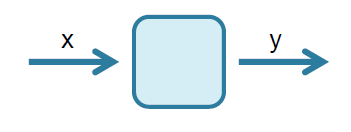
\includegraphics[width=0.4\linewidth]{fig/screenshot004}
	\label{fig:screenshot004}
\end{figure}
	\underline{Ad esempio} una bilancia del tipo ortofrutta in entrata $x$ misura il peso (grandezza meccanica) ed in uscita $y$ una variazione angolare (grandezza meccanica) che permette la visualizzazione della misura. 
	
	\underline{Ad esempio} un termometro a bulbo in entrata $x$ misura una temperatura mentre in uscita $y$ una differenza di quota $\Delta h$. \newline 
	
	Nelle ipotesi in cui il processo di trasduzione possa essere ricondotto ad un
	unico segnale di ingresso e ad un unico segnale in uscita (sarà compito dello
	sperimentatore verificare la correttezza di tale ipotesi) si può ricondurre il problema ad un legame funzionale del tipo: 
	\[ y = F(x)\]	
\begin{figure}[H]
	\centering
	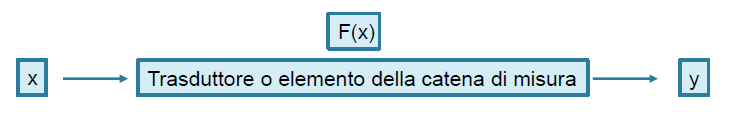
\includegraphics[width=0.5\linewidth]{fig/screenshot005}
	\label{fig:screenshot005}
\end{figure}
	Si dice che il \textbf{problema} è \textbf{di analisi} se noti $x; F(x)$ occorre valutare $y$. Questo è un problema che non entra nel campo delle misure. \newline 
	
	Si dice che il \textbf{problema} è \textbf{di sintesi} se noti $x; y$ occorre progettare il trasduttore affinché la funzione $F$ verifichi la specifica relazione funzionale $y = F(x)$.
	
	Che relazione lega l'ingresso con l'uscita? 
	
	Risolvo attraverso il processo di taratura. \newline 
	
	Si dice che il \textbf{problema} è \textbf{di misura} se noti $y; F(x)$ occorre determinare $x$, stimo ovvero il misurando attraverso la conoscenza della $F(x)$. \newline 
	
	Si può vedere il trasduttore a sua volta suddiviso in tre ulteriori blocchi: quello di captazione, sensibile all'input d'ingresso, fornisce qualcosa in uscita; quello di elaborazione, che manipola il segnale permettendone l'interpretazione (magari amplifica) e quello di rivelazione, il display che permetta la visualizzazione della misura. \newline 
	
	\textit{Ad esempio} nel termometro a bulbo la captazione è ad opera del fluido, l'elaborazione avviene attraverso lo spessore del capillare - diminuendo lo spessore aumenta il $\Delta h$ e la leggibilità della misura - e la rivelazione è possibile grazie alla scala graduata. 
	
	\textit{Ad esempio} nel manometro l'elaborazione è ad opera di un tubicino che si deforma al passaggio dell'aria, l'elaborazione avviene attraverso elementi meccanici che trasformano lo spostamento in rotazione e la rivelazione è possibile attraverso una lancetta che si muove su una scala graduata. 
	
	I trasduttori si suddividono a loro volta in più tipologie, si può avere un trasduttore: 
	\begin{itemize}
		\item \textbf{A sistema di misura zero} 
		 
		L'indicatore dà la sola informazione quando è sullo zero. Annulla l’effetto indotto dalla variabile da misurare; è un metodo di misura più preciso e più lineare, con meno isteresi o giochi.
		
		Indicato per misure statiche. Utilizzato per misurare la massa.
		
		La misura avviene per comparazione di masse campione fino a quando l'indicatore non condurrà all'equilibrio. L'esempio a lezione è la bilancia per orafi.
		
\begin{figure}[H]
	\centering
	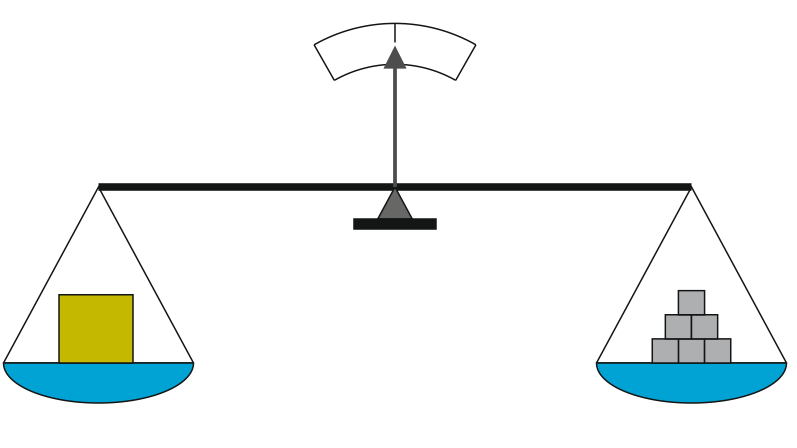
\includegraphics[width=0.3\linewidth]{fig/screenshot006}
	\label{fig:screenshot006}
\end{figure}
 		
		\item \textbf{A sistema di misura a deflessione} 
		 
		Tale sistema di misura diviene più rapido che incasellare masse campione su di un piatto finché non sopraggiunge l'equilibrio, inoltre si presta meglio del precedente a misure dinamiche. 
		
\begin{figure}[H]
	\centering
	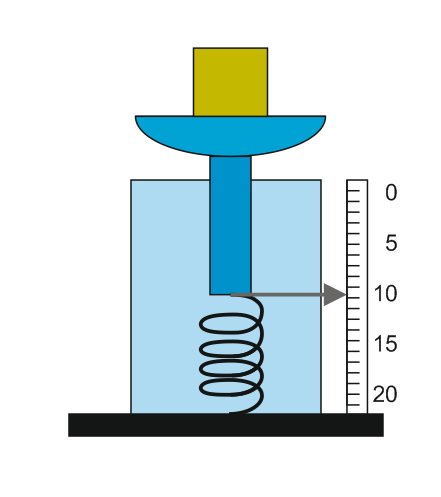
\includegraphics[width=0.3\linewidth]{fig/screenshot007}
	\label{fig:screenshot007}
\end{figure}


		\item \textbf{Passivo} 
		 
		In cui le uniche due porte verso l'esterno sono quelle di ingesso ed uscita e l'energia per effettuare la misurazione è fornita dallo stesso misurando.
		
		\item \textbf{Attivo} 
		 
		In cui oltre alle due porte di ingresso e uscita è necessaria un'altra porta destinata al rifornimento di energia. 		
	\end{itemize}

	Un trasduttore può essere considerato
	come un oggetto multi-input e multi-output, specialmente quando l'output può risentire e variare in base alle condizioni ambientali. 
	
\newpage 
	
	\underline{Esempio: termometro a resistenza}
\begin{figure}[H]
	\centering
	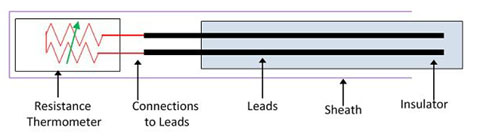
\includegraphics[width=0.5\linewidth]{fig/screenshot008}
	\label{fig:screenshot008}
\end{figure}
	Dotato di trasduttore attivo, in un termometro a resistenza l'input $x$ è la temperatura o la sua variazione, mentre l'output $y$ è una variazione di resistenza che manipolata permette di leggere una variazione di temperatura. 
	
	Un termometro a resistenza è tale per cui, fornendo una corrente $ I  $ si misura una differenza di potenziale $ \Delta V $ dalle quale ci si può ricondurre a:
	\[ R=\dfrac{\Delta V}{I}\]
	Ma:
	\[ R = \rho \dfrac{l}{S}\]
	Cosa succede se traziono il provino a cui è applicato questo termometro? Traziono anche il sensore del termometro, variando le sue caratteristiche geometriche la resistenza che misurerà non sarà più quella reale ma sarà la somma di una componente reale ed di una grandezza di  influenza:
	\[\Delta R = \Delta R_T + \Delta R_\varepsilon\]
	Ciò che infine si misurerà sarà una variazione di temperatura somma di una variaizone reale più una variazione virtuale:
	\[\Delta T = \Delta T_T + \Delta T_\varepsilon \]
	
	\underline{Esempio: estensimetro} 
	
	Un estensimetro misura la deformazione ed è sostanzialmente uguale ad un termometro a resistenza, cambia soltanto il materiale del resistore. 
	
	In questo caso il misurando $x$ è $\varepsilon$ mentre l'output è $\Delta R$. 
	
	Mettendo ora il provino a cui è applicato questo estensimetro in un ambiente soggetto a differenze di temperatura, e sapendo che la resistenza di un materiale varia con la temperatura, anche in questo caso si misurerà una resistenza dovuta al fattore reale, ovvero all'estensione più una resistenza dovuta alla differenza di temperatura, questa grandezza di influenza:
	\[\Delta R = \Delta R_\varepsilon + \Delta R_T  \] 
	E il misurando si presenterà come somma di una misura vera più una misura virtuale: 
	\[ \varepsilon = \varepsilon_\varepsilon + \varepsilon_T\]
	Invertendo i risultati ottenuti nello scorso esempio.
	\end{adjustwidth} 
	 
\newpage
	
\section{Caratteristiche metrologiche statiche}  
\begin{adjustwidth}{2in}{}
	Con caratteristiche statiche si intende l'insieme delle proprietà metrologiche
	che consentono una completa descrizione del funzionamento di un
	trasduttore o elemento della catena di misura, operante in specifiche
	condizioni ambientali quali:
	\begin{itemize}
		\item Variazioni lente del misurando;
		\item Assenza di shock, vibrazioni ed accelerazioni (a meno che tali grandezze siano
		l'oggetto della misura);
		\item Condizioni ambientali per cui:
		\begin{itemize}
			\item $T\in[15\degree C \div 35\degree C]$
			\item $UR \le 90\%$
			\item $P\in[90kPa \div 110kPa]$
		\end{itemize}
	\end{itemize}
	L'ingesso è dunque statico, fisso, e se varia lo fa molto lentamente. 
	
\begin{enumerate}
\item \textbf{Curva di graduazione} 

	Corrisponde alla legge fisica su cui si basa il metodo di misura.  
	
	\underline{Per una bilancia a piatto} entra una forza ed esce un angolo che indica il peso di tale oggetto.	
\begin{figure}[H]
	\centering
	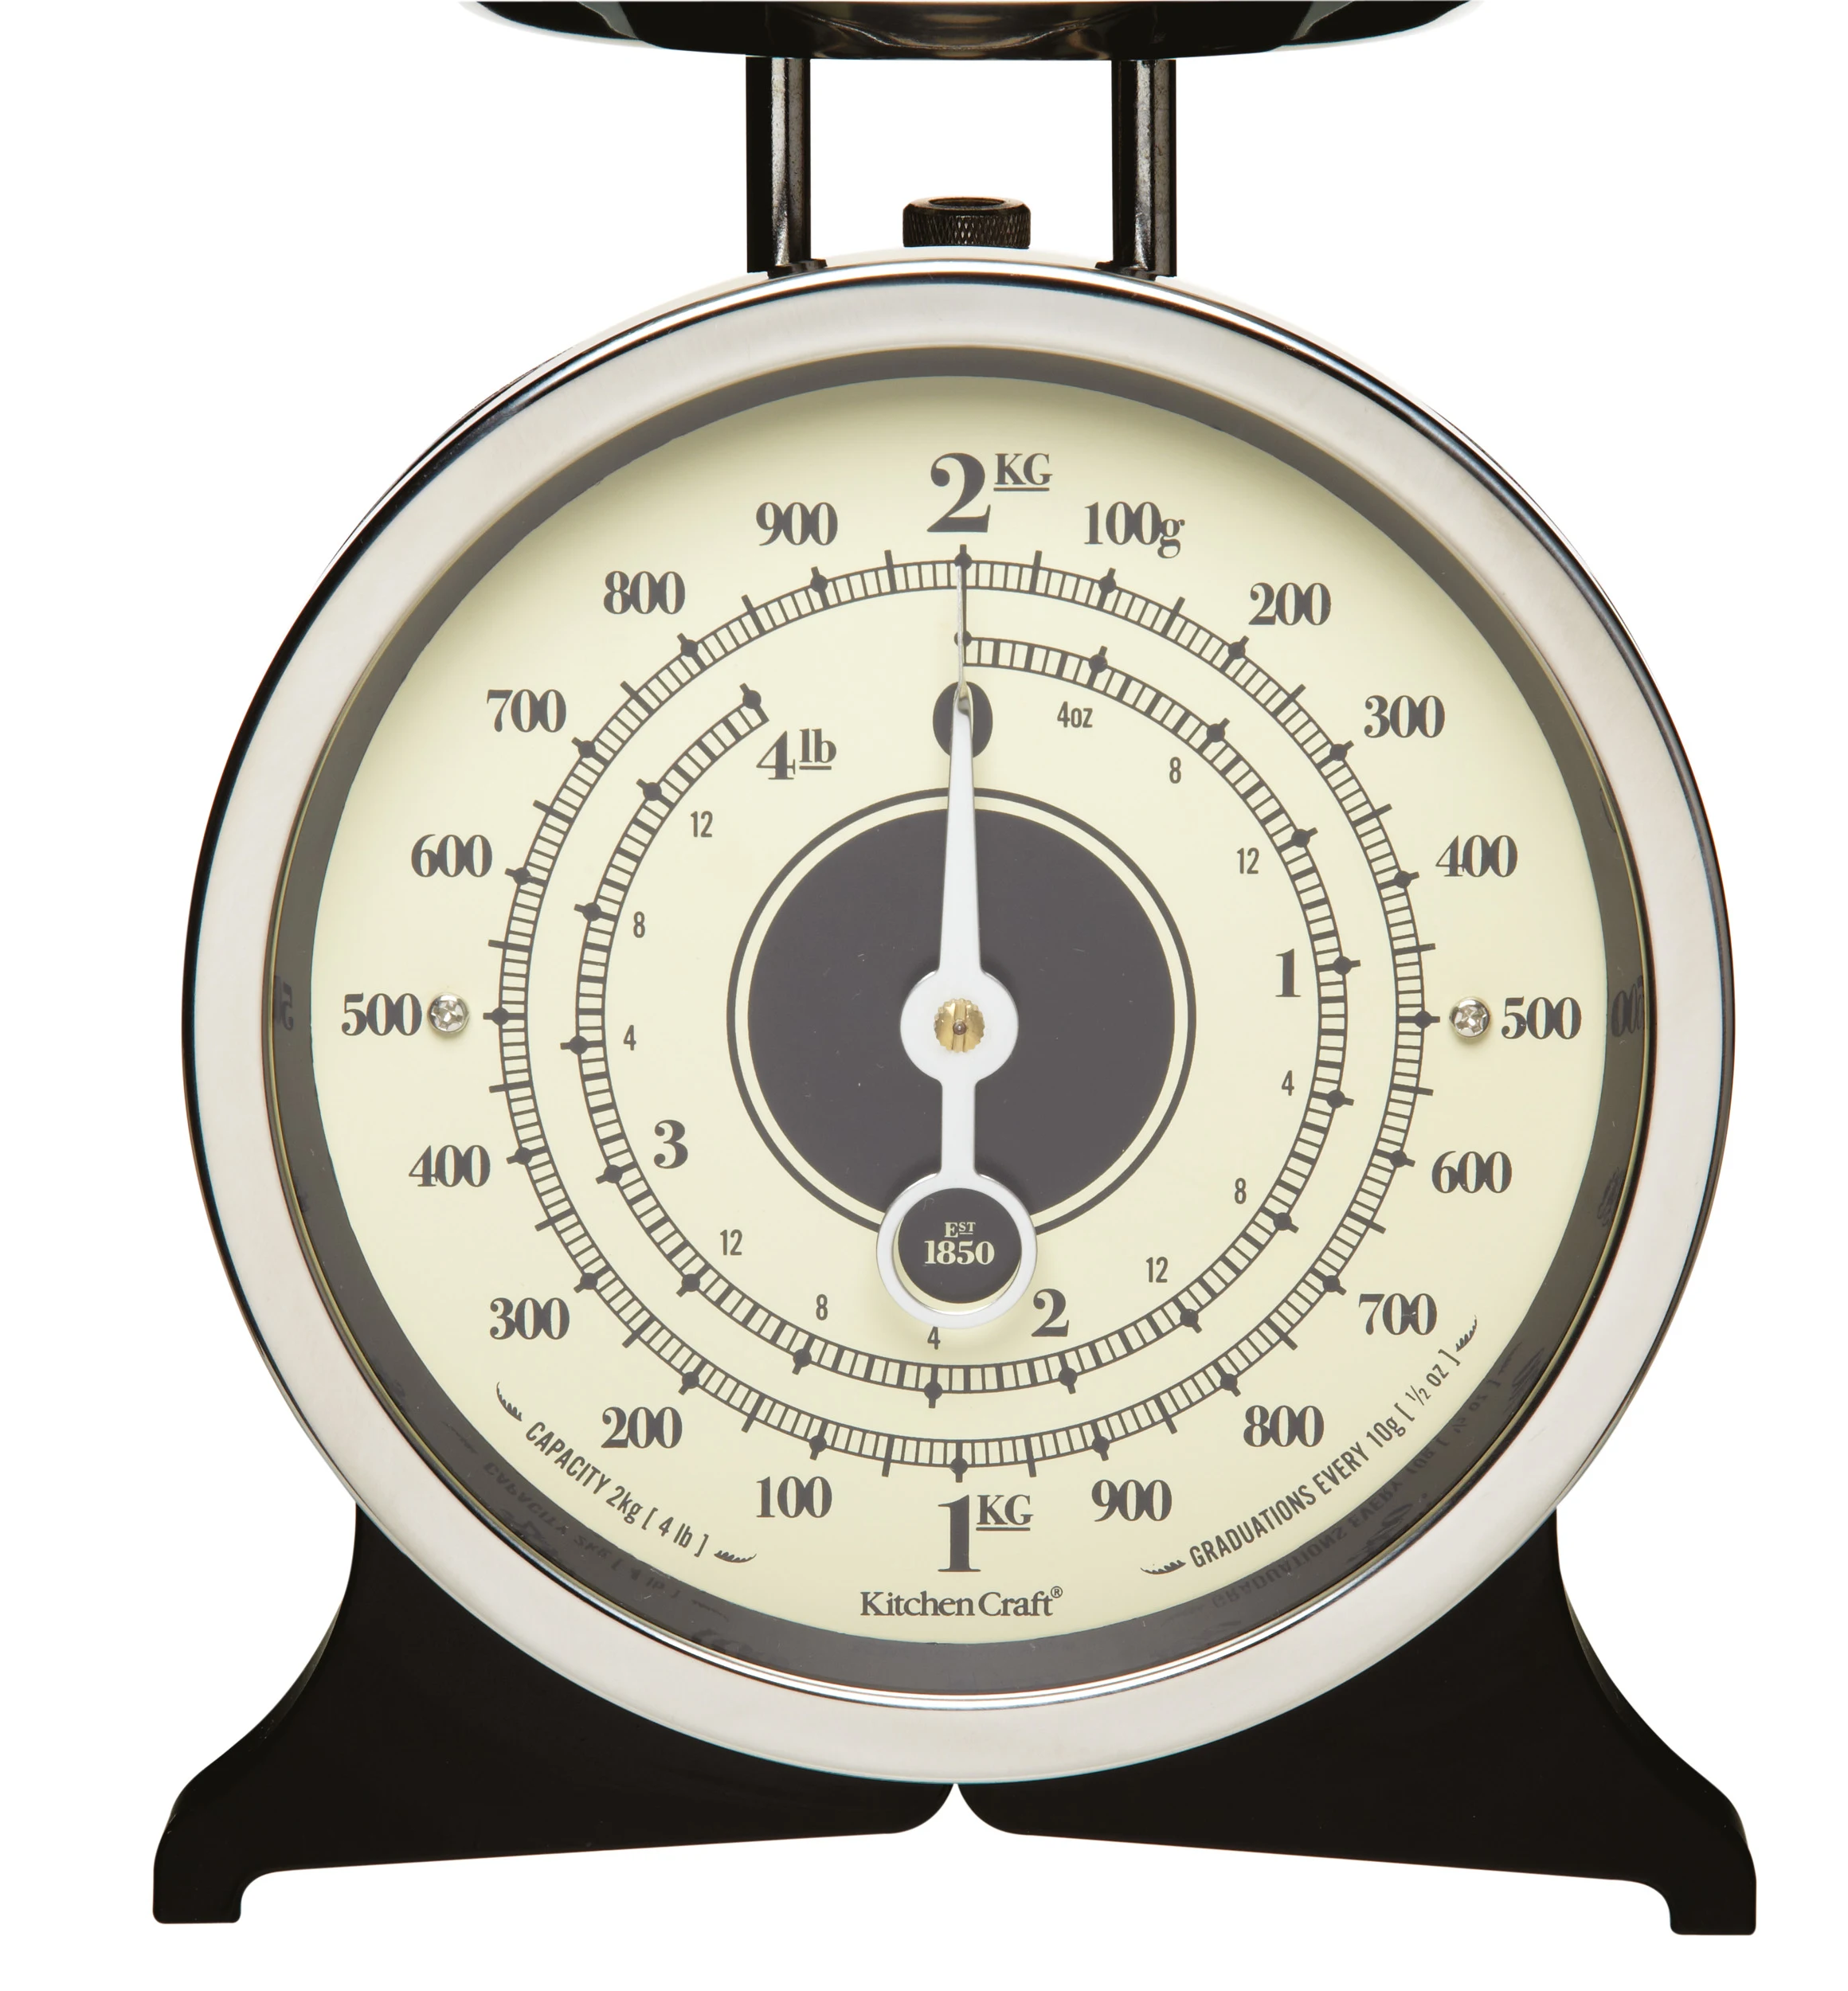
\includegraphics[width=0.3\linewidth]{fig/M22159844_3}
	\label{fig:m221598443}
\end{figure}
	\[ \begin{dcases}
		F = kz: ~ \text{Legge di Hooke} \\
		\alpha = \lambda Z: ~ \text{Legame angolare tra la diminuzione di quota e l'angolo visualizzato}
	\end{dcases}\]
	Nella curva di graduazione compaiono le equazioni fisiche che legano ingresso e uscita. 
	\[ F = k\dfrac{\alpha}{\lambda}\]
	
	\underline{Per un termometro a bulbo} entra una variazione di temperatura ed esce una variazione di quota. 	
\begin{figure}[H]
	\centering
	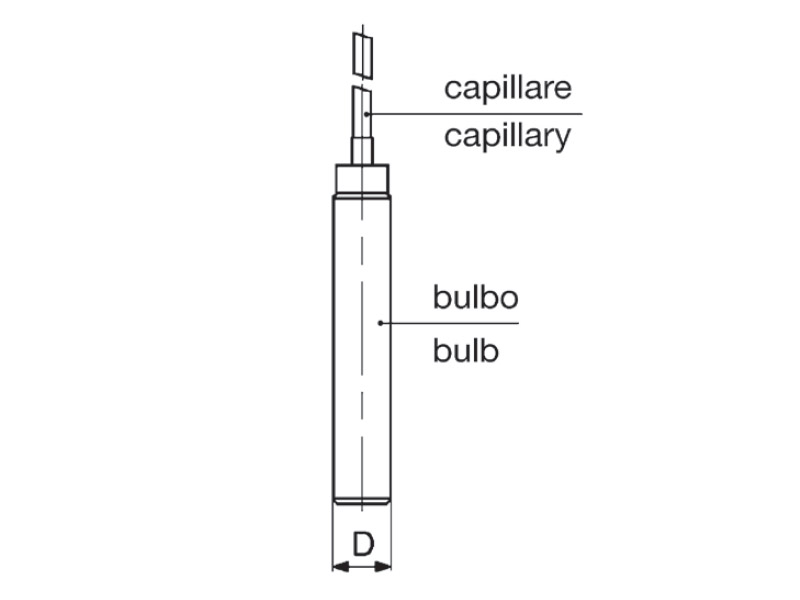
\includegraphics[width=0.3\linewidth]{fig/bulbo}
	\label{fig:bulbo}
\end{figure} 
	La variazione del volume del fluido nel termometro è data da: 
	\[\dfrac{\Delta V}{V_i} = \alpha \Delta T\]
	Ma: 
	\[\Delta V = \dfrac{a\Delta h}{V}\]
	Con $a$ sezione del capillare.
	
	Dunque la curva di graduazione sarà identificata da:
	\[ \Delta h = \dfrac{V\alpha \Delta T}{a}\]	
	NB: Quello che interessa ai fini della misura è il $\Delta T$, dunque, si applicherà l'inverso. 
	
\item \textbf{Curva di taratura} 

	La curva di taratura si determina sperimentalmente, è totalmente empirica. \newline 
	
	Si traccia per punti e rappresenta la differenza tra la misura $u$ del campione e la misura $u_b$ dello strumento da tarare, in funzione di $u_b$. \newline 
	
	\underline{Bilancia a piatto} 
	
	Si trova una relazione empirica tra la forza applicata, che deve essere nota, e l'angolo di variazione della lancetta. 
	
	Quello che si ottiene è una retta di interpolazione/regressione lineare della misura di più dati.	
\begin{figure}[H]
	\centering
	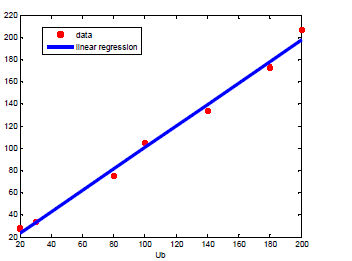
\includegraphics[width=0.5\linewidth]{fig/screenshot009}
	\label{fig:screenshot009}
\end{figure}

	\underline{Termometro a bulbo }
		
	Per un termometro si può imporre una temperatura nota attraverso una camera termostatica e misurare l'altezza alla quale si porta il fluido, caso per caso.
	
	Volendo, essendo la temperatura della camera termostatica nota, si possono fare considerazioni anche sulla misura di questa temperatura da parte del termometro e \textit{plottare} in questo modo una differenza di temperatura in funzione della temperatura dello strumento da tarare, in questo modo si ottiene una curva che identifica le sezioni in cui occorre correggere la misura.  	
\begin{figure}[H]
	\centering
	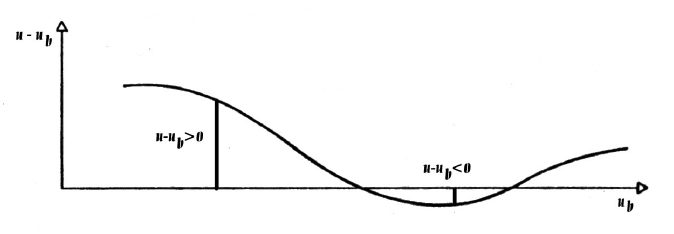
\includegraphics[width=0.5\linewidth]{fig/screenshot010}
	\label{fig:screenshot010}
\end{figure}

\newpage

\item \textbf{Campo di misura} 

	Il campo di misura è  quell'intervallo di valori della grandezza in ingresso (definito dalla portata massima e
	minima) all'interno del quale il trasduttore possiede le caratteristiche metrologiche
	dichiarate dal costruttore: fuori da tale campo l'incertezza di misura sale e le caratteristiche dello strumento non sono più soddisfatte e garantite. \newline 
	
	Si definiscono:
	\begin{itemize}
		\item \textbf{Portata minima}: valore della grandezza da misurare al di sotto della quale lo strumento
		fornisce indicazioni con incertezza maggiore di quella dichiarata;
		\item \textbf{Portata massima}: valore della grandezza da misurare al di sopra della quale lo
		strumento fornisce indicazioni con incertezza maggiore di quella dichiarata;
		\item \textbf{Portata}: portata massima quando la portata minima è pari a zero;
		Sovraccarico nominale: valore massimo consentito per la grandezza da misurare oltre il
		quale lo strumento subisce danni
		\item \textbf{Campo di sicurezza} (per il misurando): Intervallo comprendente tutte le misure del misurando cui un dispositivo per
		misurazione può essere applicato senza che il suo diagramma di taratura
		resti permanentemente alterato. 
		
		Tale campo di sicurezza dev'essere più ampio del campo di misura per garantire all’operatore un ragionevole margine di sicurezza nei confronti di
		alterazioni permanenti dei risultati della taratura, che potrebbero portare a
		misure non compatibili.
		
		Qualora un dispositivo per misurazione sia stato applicato a misurandi le cui
		misure siano al di fuori del campo di sicurezza, è necessario eseguire una
		verifica della taratura.
		
	\end{itemize}
	In sostanza (1) all'interno del \textit{Limit load} è consigliabile ritarare lo strumento; (2) lo strumento può funzionare anche oltre al \textbf{Breaking load} perché magari può deformarsi plasticamente, ma sarà ora fonte di errori sistematici. 	
	
\begin{figure}[H]
	\hspace{-1cm}
	\centering
	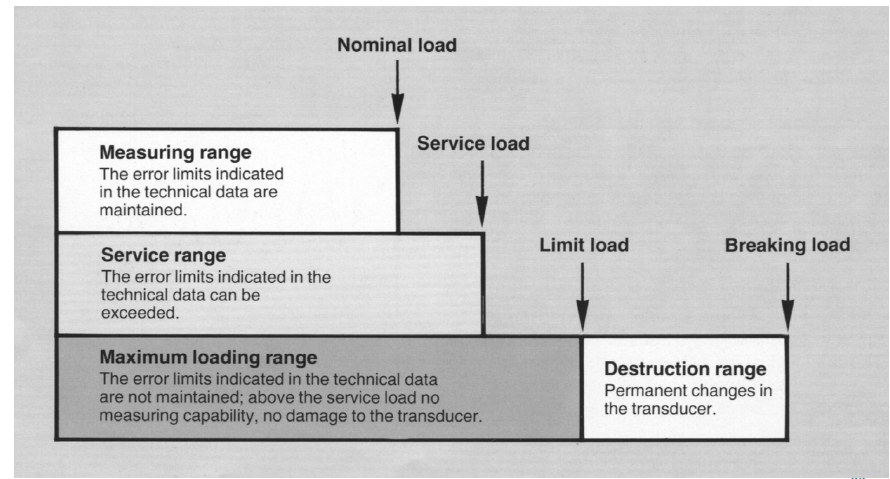
\includegraphics[width=1\linewidth]{fig/screenshot011}
	\label{fig:screenshot011}
\end{figure}

\newpage

\item \textbf{Sensibilità, guadagno, \textit{gain}} 

	La sensibilità è l’attitudine/capacità dello strumento nel rilevare “piccole” variazioni della grandezza in ingresso ed è la derivata della curva di graduazione, il suo coefficiente angolare, la sua pendenza. 
	\[ S = \dfrac{dy}{dx} = \left[\dfrac{y}{x} \right] \]
	Si definiscono se la derivata è rispettivamente costante, lineare o inversa, strumenti:
	\begin{itemize}
		\item Lineari 
		\[y = kx \Rightarrow S = k\]
		La sensibilità migliore, ideale si avrà quando si riusciranno a valutare le più piccole variazioni del segnale in ingresso ovvero a piccoli intervalli della grandezza in ingresso corrisponderanno grandi intervalli di output, ci troveremo in questo caso sulla bisettrice. \newline
		
		Uno strumento lineare ha come punto di forza la sensibilità costante, ovvero all'interno del campo di misura risponde alla variazione del misurando sempre nello stesso modo.
		
		\item Quadratici 
		\[y = kx^2 \Rightarrow S = 2kx\]
		Uno strumento di questa tipologia presenza non più una sensibilità costante, ma sarà molto sensibile per valori molto alti, piuttosto che per valori bassi, simili allo zero. 
		
		Un esempio può essere fornito dal tachimetro dell'automobile. 
		
		\item Logaritmici
		\[ y = \log x \Rightarrow S = k/x\]
		Questo invece molto sensibile per valori prossimi allo zero. 
	\end{itemize}

\item \textbf{Linearità} \newline
	Questa caratteristica risponde alla domanda, quanto uno strumento può essere approssimato o considerato come lineare? \newline 
	
	Se per lo strumento di misura considerato pongo la misura $0=0\%$ e la misura al fondo scala $FS = 100\%$, la linearità è in questo modo definita come percentuale di scostamento
	dal comportamento del sensore ed è funzione del criterio statistico utilizzato per
	il calcolo della retta di linearità. \newline 
	
	Si definisce l'errore di linearità come la distanza verticale tra il massimo scostamento (singolo punto) dei punti riottenuti, diviso il fondo scala, percentualmente: 
	\[\varepsilon_{lin} = \dfrac{|Y_i - Y^*_i|_{max}}{FS}\cdot 100\]	
\begin{figure}[H]
	\centering
	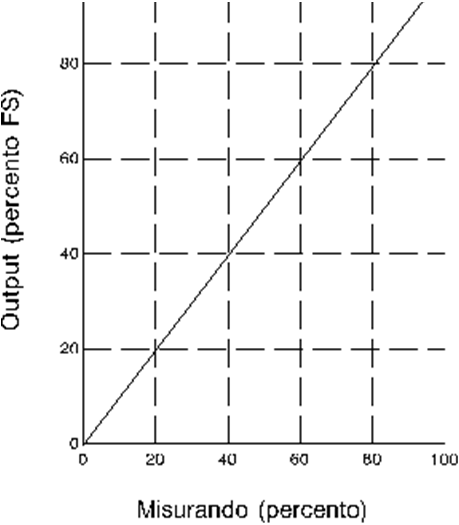
\includegraphics[width=0.3\linewidth]{fig/screenshot012}
	\label{fig:screenshot012}
\end{figure}
\begin{figure}[H]
	\centering
	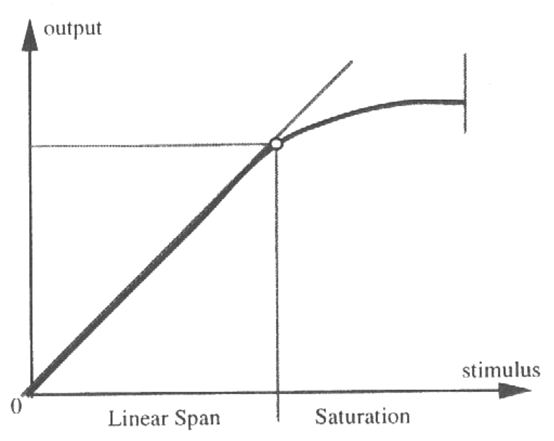
\includegraphics[width=0.3\linewidth]{fig/screenshot013}
	\caption{Dopo un certo valore, ad un intervallo di input corrisponde un output costante, una funzione costante produce derivata nulla è la sensibilità dello strumento è così nulla.}
	\label{fig:screenshot013}
\end{figure}
\begin{figure}[H]
	\centering
	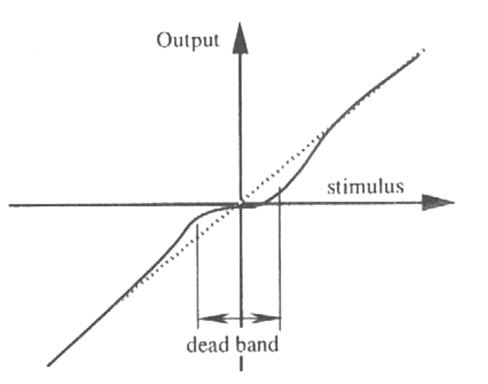
\includegraphics[width=0.3\linewidth]{fig/screenshot014}
	\caption{Curva di graduazione
		lineare solo in alcune zone}
	\label{fig:screenshot014}
\end{figure}

\item \textbf{Errore sistematico} 

	Per un errore sistematico è	nota la relazione funzionale tra l’entità dell’errore e l’intensità della grandezza fisica
	che lo genera. Si conosce l'errore, la fonte dell'errore e può essere così facilmente  eliminato.
	
\item \textbf{Errore casuale} 

	Per un errore casuale non è invece nota la legge tra la causa dell'errore e l’effetto che genera nella misurazione. Poiché non può essere eliminato perché non è più frutto di una sistematicità ma di una casualità, tale errore deve essere ridotto.
	
\item \textbf{Giustezza - Goodness} 

	Grado di concordanza tra la media di un numero infinito di
	valori misurati ripetuti e un valore di riferimento, quantifica la prossimità del valore medio al valore “vero” della
	misura: Quanto il valore medio si distanzia dal valore vero? 
	
	È Legata agli errori sistematici, se non sono stati eliminati tale distanza aumenta.
	
\item \textbf{Precisione} 

	Grado di concordanza tra i valori misurati ottenuti da un certo
	numero di misurazioni ripetute. È indice del grado di dispersione un insieme di
	dati sperimentali. Viene valutata prendendo in considerazione la deviazione
	standard, se questa è elevata il valore vero devia altrettanto. È Legata agli errori casuali.
\newpage	
\item \textbf{Accuratezza} 

	Grado di concordanza tra un valore misurato ed il valore vero
	del misurando: come si rapporta la singola misura rispetto al valore vero? 
	
	È influenzata da entrambi gli errori. 	
\begin{figure}[H]
	\centering
	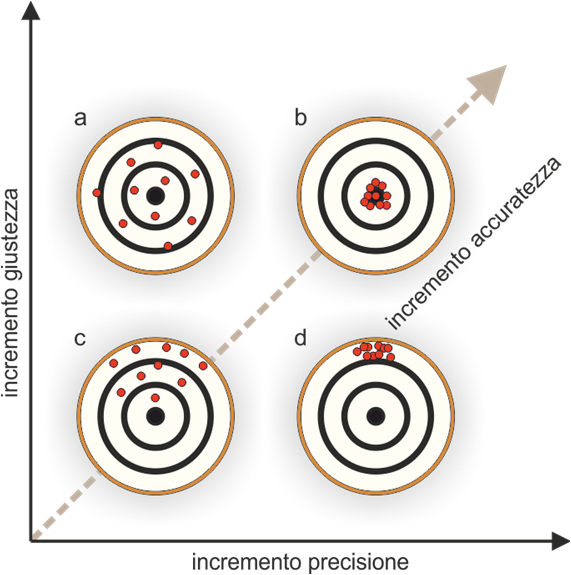
\includegraphics[width=0.5\linewidth]{fig/screenshot015}
	\label{fig:screenshot015}
\end{figure}

\item \textbf{Isteresi} 

	Frequente negli strumenti in cui si misurano pesi o forze in generale. \newline 
	
	A titolo esemplificativo si pongano su una bilancia a piatto delle masse via via crescenti fino a raggiungere il fondo scala, ci si ponga poi nel caso di dover misurare un intervallo di variazione di peso, ci si chiede: questo intervallo di misure è uguale a quello che ottengo levando massa fino a raggiungere lo zero, ovvero procedendo dall'alto piuttosto che dal basso? No, l'output può variare a causa di giochi meccanici presenti nello strumento. 	
\begin{figure}[H]
	\centering
	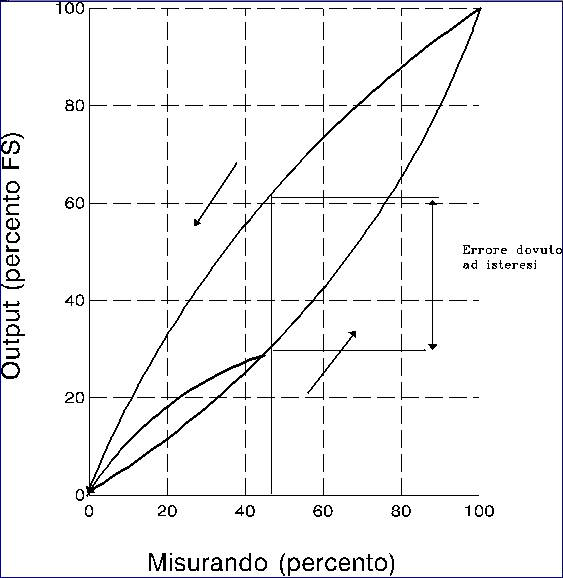
\includegraphics[width=0.5\linewidth]{fig/screenshot016}
	\label{fig:screenshot016}
\end{figure}
	L'isteresi si configura così essere la differenza massima tra il valore rilevato dal trasduttore quando viene applicato uno
	specifico valore della grandezza in ingresso raggiunto imponendo ingressi crescenti,
	ed il medesimo valore ottenuto imponendo ingressi decrescenti. \newline
	
	L'errore di isteresi è la stima della massima distanza tra la due strade percorse:
	\[\varepsilon_{ist} = \dfrac{|Y^S_i - Y^D_i|_{max}}{FS}\cdot 100\]
	
\item \textbf{Errore di inserzione} 

	Attitudine di uno strumento a non perturbare la grandezza oggetto della
	misura:
	\[\varepsilon_{ins} = \dfrac{|y_m - y_v|}{y_m}\]
	In cui $y_v$ è il valore vero e $y_m$ è il valore misurato in presenza dello strumento di misura. \newline 
	
	Ad esempio un termometro a bulbo in una grande vasca d'acqua raggiungerà dopo un certo tempo l'equilibrio termico e la lettura della temperatura sarà il più possibile vicino a quella reale, lo stesso tipo di termometro all'interno di una tazzina d'acqua assorbirà "troppo" calore dall'acqua per portarsi in equilibrio termico, falsando inevitabilmente la misura.
	\begin{itemize}
		\item \textit{Misura di tensione} 
		
		Un voltmetro reale in parallelo ad un ramo che possiede una propria resistenza ne misura la tensione ai suoi capi. 
\begin{figure}[H]
	\centering
	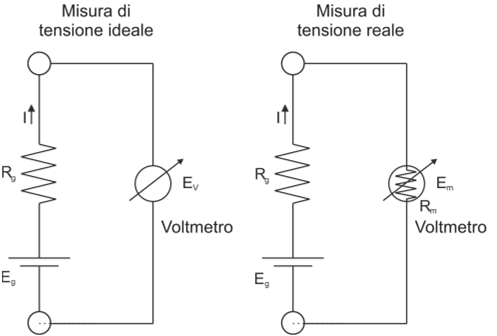
\includegraphics[width=0.5\linewidth]{fig/screenshot017}
	\label{fig:screenshot017}
\end{figure}
		Il voltmetro chiuso sul ramo possiede una propria resistenza ed un proprio generatore (è composto da un trasduttore attivo) e forma una maglia chiusa per cui: 
		\[ E_m = I R_m = E_g - IR_g \Rightarrow I = \dfrac{E_g}{R_m + R_g}\]
		\[ E_m = E_g \dfrac{R_m}{R_m + R_g} \] 
		\[\varepsilon_{ins} = \dfrac{|y_m - y_v|}{y_m} = \dfrac{E_m - E_v}{E_m} = 1- \dfrac{E_g}{E_m} = 1- \dfrac{R_m + R_g}{R_m}  = \dfrac{R_g}{R_m} \] 
		\[\varepsilon_{ins} = \dfrac{R_g}{R_m} \Rightarrow R_m >> R_g \]
		Affinché si ottenga una misura della tensione più veritiera possibile, la resistenza del voltmetro dev'essere molto più grande della resistenza propria del ramo.
\newpage		
		\item \textit{Misura di corrente} 
		
		Un amperometro reale in serie ad un ramo che possiede una propria resistenza ne misura la corrente che scorre attraverso esso.		
\begin{figure}[H]
	\centering
	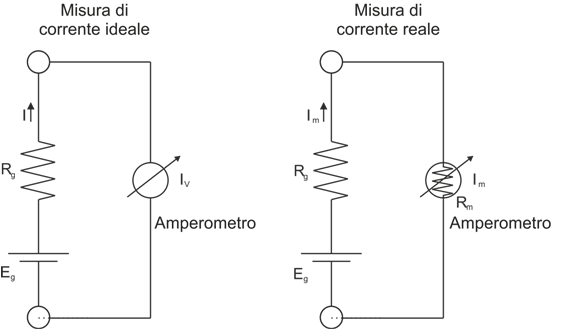
\includegraphics[width=0.5\linewidth]{fig/screenshot018}
	\label{fig:screenshot018}
\end{figure}
	La corrente circola solo su maglie chiuse, in questo modo possedendo l'amperometro  una propria resistenza ed un proprio generatore (è composto da un trasduttore attivo), si nota che: 
	\[I_m = I; E_g = I_vR_g \]
	\[E_g = I_m(R_g + R_m)\]
	\[I_vR_g = I_m(R_g + R_m)\]
	\[\varepsilon_{ins} = \dfrac{|y_m - y_v|}{y_m} = \dfrac{I_m - I_v}{I_m} = 1- \dfrac{I_v}{I_m} = 1- \dfrac(R_g + R_m){R_g}  = \dfrac{R_m}{R_g} \] 
	\[\varepsilon_{ins} = \dfrac{R_m}{R_g} \Rightarrow R_g >> R_m \]
	Affinché si ottenga una misura della corrente più veritiera possibile, la resistenza dell'amperometro dev'essere molto più piccola della resistenza propria del ramo.
	
	\item \textit{Dinamometro} 
	\begin{figure}[H]
		\centering
		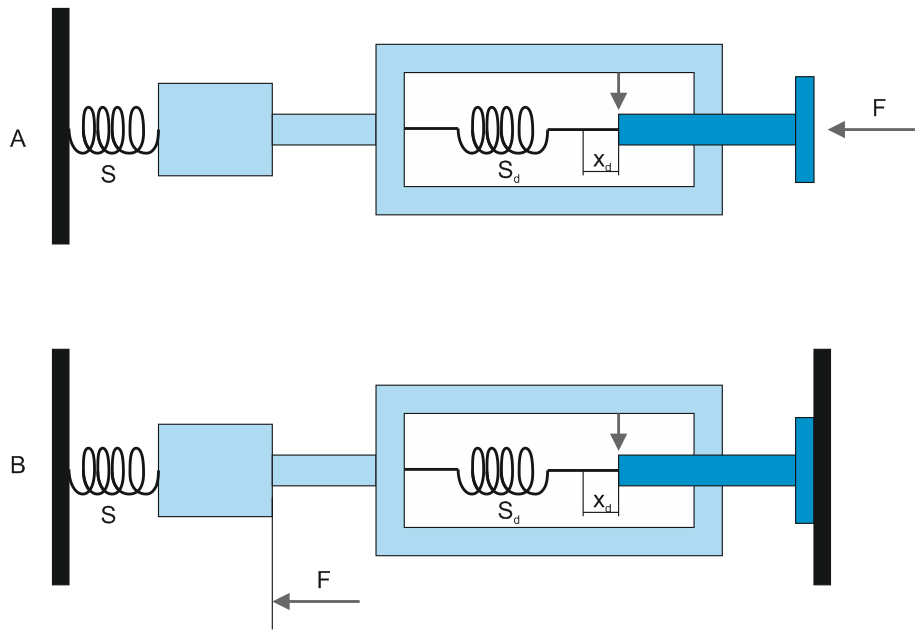
\includegraphics[width=0.5\linewidth]{fig/screenshot019}
		\label{fig:screenshot019}
	\end{figure}
		\begin{itemize}
			\item Errore di inserzione nullo: dinamometro libero			
			\[F_m = F \quad \varepsilon_{ins} = \dfrac{F_m-F_v}{F_m} = 0\]
			\item Presenza di errore di inserzione: dinamometro vincolato
			\[F_m = S_d\cdot x_d\]
			\[F=F_v = S\cdot x_d + S_d\cdot x_d\]
			\[\dfrac{F_m-F_v}{F_m} = 1 - \dfrac{F_v}{F_m} = 1 - \dfrac{S+S_d}{S_d} = \dfrac{S}{S_d}\]
			\[S_d\gg S\]
		\end{itemize}
	\item \textit{Comparatore} 
	Un comparatore misura il grado di rugosità superficiale, è una punto con una molla che segue il profilo dell'oggetto. \newline
	
	Si intende in questo caso calcolare la deformazione della molla. ($S$ costante elastica).
	
\begin{figure}[H]
	\centering
	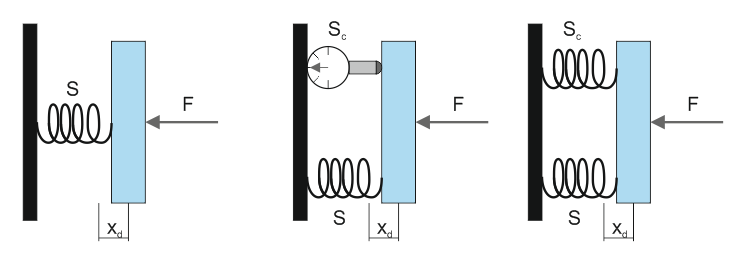
\includegraphics[width=0.5\linewidth]{fig/screenshot020}
	\label{fig:screenshot020}
\end{figure}

	Ma il comparatore è già una molla! Misuro la deformazione anche di un'altra molla!
	\[ x_v = F/S; x_m = \dfrac{F}{S + S_c}\]
	Ricordando che due molle in parallelo si sommano. 
	
	Si arriva infine a:
	\[\varepsilon_{ins} = \dfrac{|y_m - y_v|}{y_m} = \dfrac{x_m - x_v}{x_m} = 1- \dfrac{x_v}{x_m} = 1- \dfrac(S + S_c){S}  = \dfrac{S_c}{S} \] 
	\[\varepsilon_{ins} =  \dfrac{S_c}{S} \Rightarrow S_c << S \]
	Affinché si ottenga una misura della deformazione della molla più veritiera possibile, la costante elastica del comparatore dev'essere molto più piccola della costante elastica della molla che si intende misurare.	
	\end{itemize}

\item \textbf{Ripetibilità} 

	Attitudine di uno strumento a fornire \underline{valori di lettura poco differenti} tra di loro,
	\underline{in letture consecutive eseguite} indipendentemente \underline{sullo stesso misurando},
	con procedimento unificato, \underline{dallo stesso operatore}, \underline{nelle stesse condizioni}
	per le grandezze d'influenza.
	
	[UNI 4546, 6.3]
	
\item \textbf{Riproducibilità} 

	\underline{Variazione tra le medie delle misure}, \underline{\textbf{effettuate da differenti}} \\ \underline{\textbf{operatori che
	utilizzano diversi strumenti}}per misurare lo stesso parametro. \newline 

	Rispetto alla ripetibilità viene sostituito l'operatore e lo strumento. \newline 
	
	Se l'intervallo di riproducibilità è maggiore di quello della ripetibilità nel caso su usi lo
	stesso strumento si effettueranno per gli operatori dei training sulle modalità di utilizzo e di lettura
	delle apparecchiature di prova e collaudo. \newline
	
	Se l'intervallo di ripetibilità è maggiore di quello della riproducibilità si effettuerà o
	incrementerà la manutenzione delle apparecchiature. 
	
\item \textbf{Stabilità} 

	Attitudine di uno strumento a fornire \underline{valori di lettura poco differenti} tra di loro,
	\underline{in letture eseguite} indipendentemente, \underline{sullo stesso misurando}, \underline{\textbf{in un intervallo
	di tempo definito}}, con procedimento unificato e nelle stesse condizioni per le
	grandezze d'influenza.
	
	[UNI 4546, 6.4]
	
	\newpage 
	
	\textbf{Ripetibilità vs Stabilità} 
	
	Il valore della ripetibilità viene determinato esaminando i risultati ottenuti da
	misurazioni ripetute in successione (una subito dopo l'altra) mentre il valore della stabilità è riferito ai risultati ottenuti da misurazioni ripetute in un
	lungo arco di tempo (ad esempio tre mesi, un anno, due anni o più) e,
	comunque, da specificarsi.
	
\item \textbf{Affidabilità} 

	L'affidabilità è la capacità di uno strumento di rispettare le specifiche di
	funzionamento nel tempo.
	
	Raramente viene indicata nei data sheet ed è espressa come MTBF \textit{mean
	time between failures}. \newline
	
	Per parlare di affidabilità è necessario introdurre:
	\begin{itemize}
		\item Critical failures: si perde completamente la funzionalità del dispositivo;
		\item Major failures: si perde la principale funzionalità del dispositivo ma esso può
		continuare a funzionare erogando parzialmente le sue funzioni;
		\item Minor failures: il dispositivo perde alcune funzionalità accessorie ma quelle
		principali sono mantenute
	\end{itemize}
	Poiché il MTBE può essere lungo da aspettare, per accelerare i tempi, nelle stesse condizioni di output si fa operare lo strumento nelle peggiori condizioni di esercizio in modo da accelerarne il tempo di rottura e avere dei dati in proporzione secondo formule empiriche, ad esempio per un termometro:
	\[n = N\left( \dfrac{\Delta T_{max}}{\Delta T_{test}}\right)^{2.5} \] 
	In cui $n$ è il numero di cicli da effettuare, $N$ è il numero di cicli previsti di vita, $\Delta T_{max}$  è la differenza massima della temperatura rispetto a quella ambiente
	durante la vita del trasduttore e $\Delta T_{test}$ è la differenza massima della temperatura rispetto a quella ambiente
	durante i test accelerati.\newline 
	
	Se la vita prevista è pari a 20000 cicli occorrerà effettuare circa 1300 cicli per
	verificare l'affidabilità dei trasduttori. \newline 
	
	Altri parametri per per valutare l'affidabilità sono: 
	\begin{itemize}
		\item MTTF \textit{Mean Time To Failures} \newline 
		È un indicatore per i dispositivi che vengono scartati al primo danneggiamento (non si
		riparano). Indica anche l’istante di tempo in cui si manifesta il secondo guasto dopo la
		riparazione;
		\item MTTR \textit{Mean Time To Repair} \newline
		È il tempo medio necessario per la riparazione di un dispositivo relativamente alla
		stessa tipologia di danno.\newline 
		
		In questo modo:
		\[MTBF = MTTF + MTTR\]
		\item \textit{Availability:}: $=\dfrac{MTTF}{MTTF + MTTR}$ \newline 
		Percentuale di tempo in cui il dispositivo è operativo.
		\item \textit{Customer satisfaction}
		\[MTBF \uparrow \hspace{1cm} MTTR \downarrow\]
	\end{itemize}

\newpage
		
\item \textbf{Risoluzione} 
 
		Attitudine di un dispositivo per misurazione e/o regolazione a risolvere stati
		diversi del misurando durante la misurazione.
		
		[UNI 4546, 6.2] \newline
		
		La risoluzione è la più piccola parte che si riesce a misurare con uno strumento, l'unità di misura è la stessa del misurando $x$. \newline
		
		In alcuni trasduttori, come il potenziometro a filo avvolto, se si varia in modo continuativo il misurando non si hanno variazioni continuative dell'output ma, ad esempio, step misurabili. \newline 
		
		Un potenziometro a filo avvolto presenta un filo conduttore spiralato intorno ad un materiale dielettrico, la lunghezza di tali avvolgimenti varieranno da $0$, in cui la resistenza sarà nulla, ad $L$, in cui la resistenza sarà massima $R$, nota, ovvero quella degli avvolgimenti; ad un palpatore, posto a distanza $x$, è dato il compito di identificare la resistenza in base allo spostamento lungo gli avvolgimenti, noto che:
		\[ R = \rho \dfrac{L}{S} \hspace{1cm} r = \rho \dfrac{x}{S}\]
		\[ \dfrac{r}{S} = \dfrac{x}{L} \Rightarrow r = \dfrac{R}{L}x\]
		Inoltre la sensibilità di tale strumento è $S = \dfrac{R}{L}$. \newline 
		
		Sperimentalmente accade che, piuttosto che essere la bisettrice dei quadranti, la funzione caratteristica presenta svariati gradini, questo si spiega perché il palpatore non tocca continuativamente tutte le spire , ma si sposta di spira in spira misurando un $	delta x$ costante: la più piccola variazione in ingresso non mi determina alcuna variazione in uscita, e proprio questa è la risoluzione. 		
\begin{figure}[H]
	\centering
	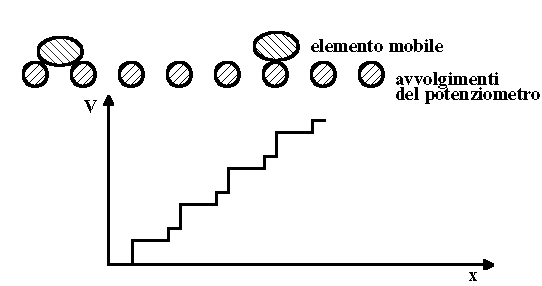
\includegraphics[width=0.5\linewidth]{fig/screenshot021}
	\label{fig:screenshot021}
\end{figure}
		Come ottengo un potenziometro che abbia una risoluzione maggiore? Aumento/infittisco il numero di spire. 
		
\item \textbf{Rumore} 
 
	Presente specialmente in misurazioni elettriche, il rumore è definito come l'insieme di variazioni casuali della grandezza da
	misurare che determinano variazioni anch'esse casuali dell'output. \newline 
	
	Può essere generato sia internamente al trasduttore e in questo caso si tratta di rumore Johnson, ossia un movimento casuale delle
	cariche che genera una f.e.m. variabile ai terminali di connessione; oppure esternalmente al trasduttore e in questo caso è dovuto a effetti di frequenza di rete, altri
	accoppiamenti magnetici, ecc. \newline 
	
	Un segnale si può vedere come periodico o pseudo-periodico e si può, attraverso le trasformate di Fourier, trasformare in segnale sinusoidale o pseudo-sinusoidale, un segnale generico altri non è che la somma di più segnali che siano periodici o non. 
	
	Un segnale in frequenza registra le ampiezze della sinusoidi, ad esempio, noto che $f = \dfrac{2\pi}{\omega}$, uno spettro del seguente segnale si scrive, con le opportune semplificazioni: 
	\[ 5\sin(2\pi t) + 2\sin(2\pi 10t)\]	
\begin{figure}[H]
	\centering
	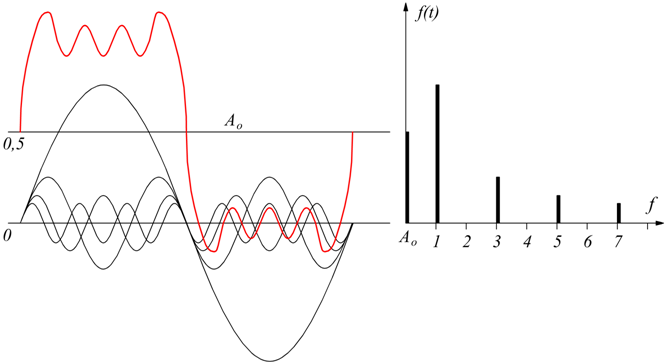
\includegraphics[width=0.7\linewidth]{fig/16}
	\label{fig:16}
\end{figure}
	Con dati rumorosi si possono applicare dei filtri che riducano o annullino il rumore, ma questo non è sempre possibile, lo è solo se il contributo in frequenza del rumore è diverso o molto lontano dal contributo in frequenza del segnale. 	
\begin{figure}[H]
	\centering
	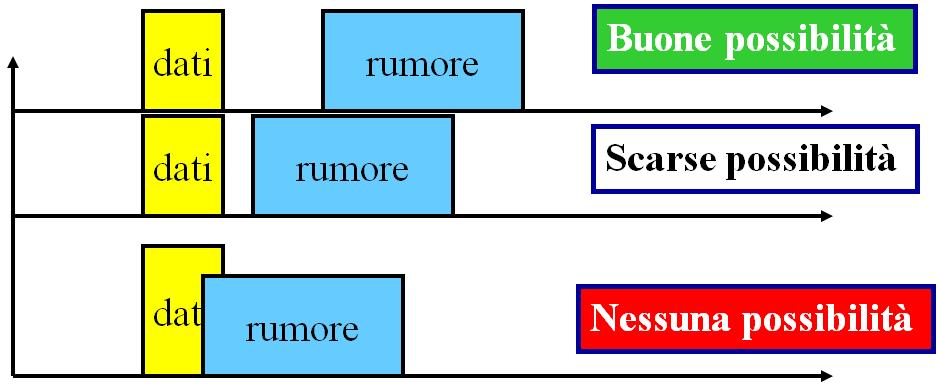
\includegraphics[width=0.5\linewidth]{fig/screenshot022}
	\label{fig:screenshot022}
\end{figure}
	\textbf{Minimo segnale rilevabile}: Ipotizzando che il segnale in ingresso al trasduttore sia privo di rumore il
	valore minimo rilevabile è funzione del livello di rumore intrinsecamente
	generato dal trasduttore stesso.		
\end{enumerate}
\end{adjustwidth}
\newpage
\subsection{Caratteristiche metrologiche statiche funzioni del tempo}	
\begin{adjustwidth}{2in}{}
	\textbf{ATTENZIONE}: NON sono caratteristiche metrologiche dinamiche, non è il misurando ad essere dinamico, sono le stesse caratteristiche a variare nel tempo. 

\begin{enumerate}
\item \textbf{Deriva di zero, \textit{offset}} 
 	
	Il trasduttore è affetto da deriva di zero se esso mostra in uscita un segnale,
	funzione del tempo, diverso da zero sotto le seguenti condizioni:
\begin{itemize}
	\item trasduttore alimentato a tensione od intensità di corrente costante;
	\item valore del misurando nullo;
	\item condizioni ambientali costanti
\end{itemize}

\begin{figure}[H]
	\centering
	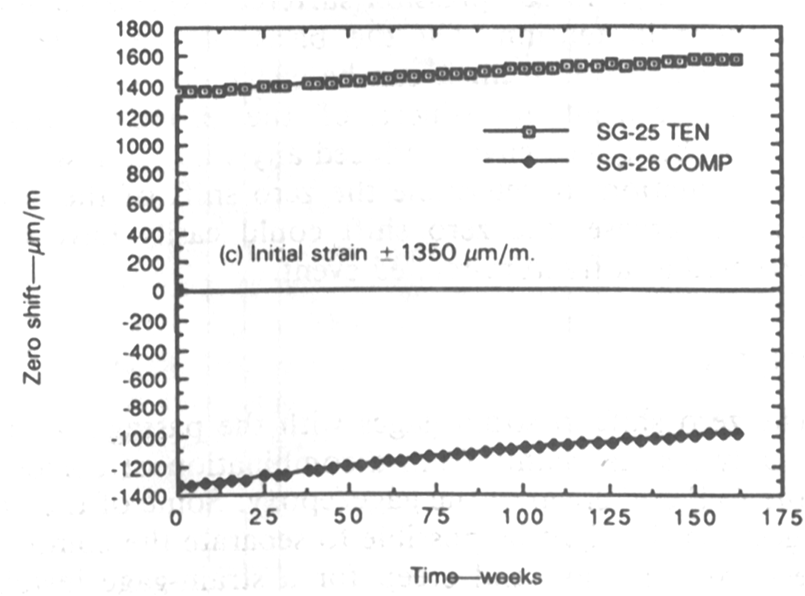
\includegraphics[width=0.5\linewidth]{fig/screenshot023}
	\label{fig:screenshot023}
\end{figure}


 L’effetto è una traslazione della curva di graduazione. 
 
  Cause? Riscaldamento del sensore, errori di calibrazione, cambiamento di temperatura, vibrazioni, isteresi...
 
 \item \textbf{Creep} 
  	
 	Il trasduttore è affetto da creep se esso mostra in uscita un segnale variabile
	sotto le seguenti condizioni:
 \begin{itemize}
 	\item trasduttore alimentato a tensione od intensità di corrente costante;
 	\item valore del misurando è costante;
 	\item condizioni ambientali costanti.
 \end{itemize}
	Molto simile alla deriva di zero, ma è formalmente legato al misurando, l'ingresso in questo caso è costante ma si registra una variazione che non si dovrebbe registrare. 
	\begin{figure}[H]
		\centering
		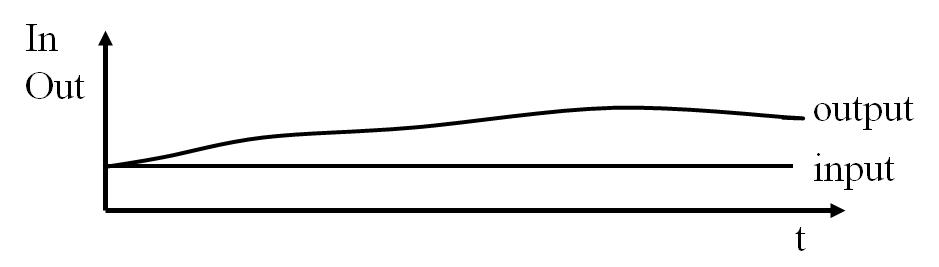
\includegraphics[width=0.5\linewidth]{fig/screenshot024}

		\label{fig:screenshot024}
	\end{figure}
\newpage	
\item \textbf{Deriva della sensibilità} 
 	
	I trasduttori possono manifestare una dipendenza della curva di graduazione
	in funzione del tempo, ossia possono variarne la pendenza e quindi la sensibilità; anche in questo caso è necessario
	indicare le condizioni ambientali alle quali sono state condotte le prove.
	
	Per una bilancia ad esempio $S=1/K$ e se cambia $K$ a causa di fattori ambientali?
	
\begin{figure}[H]
	\centering
	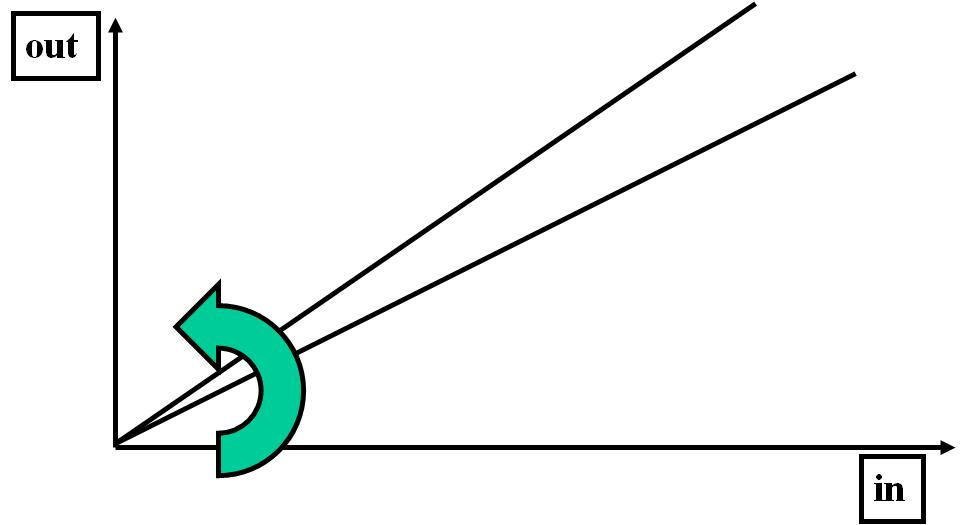
\includegraphics[width=0.5\linewidth]{fig/screenshot025}
	\label{fig:screenshot025}
\end{figure}

\item \textbf{Intervallo di errore statico e Banda di errore} 
 	
 	L'intervallo di errore statico condensa in un grafico le caratteristiche metrologiche statiche. \newline 
 	
 	La banda di errore è un intervallo di deviazione massima dell’output del trasduttore da una curva di
 	riferimento. 
 	
 	Tale deviazione deve essere causata dal trasduttore stesso ed è espressa in percentuale del Fondo Scala ($\%FS$) e tiene conto
 	dell’errore di isteresi, della non linearità, della non ripetibilità, ecc.
 	
 	La banda viene determinata con cicli di taratura consecutivi così da includere
 	anche la ripetibilità.
 	
\begin{figure}[H]
	\centering
	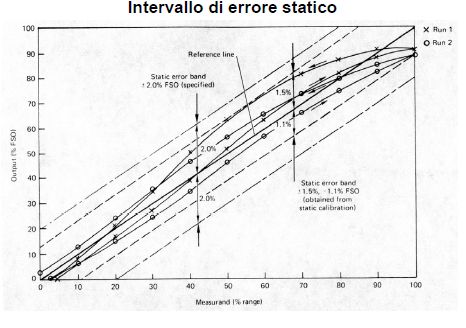
\includegraphics[width=0.5\linewidth]{fig/screenshot026}
	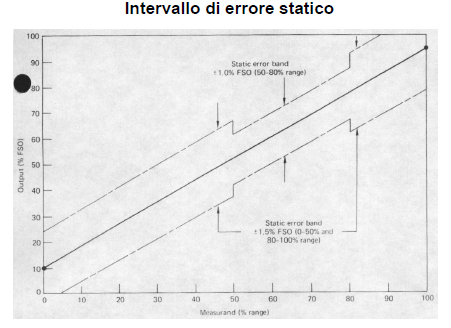
\includegraphics[width=0.5\linewidth]{fig/screenshot027}
	\label{fig:screenshot026}
\end{figure}
\end{enumerate}


\end{adjustwidth}
\newpage
\section{Grandezze di influenza}	
\begin{adjustwidth}{2in}{}
	Le grandezze di influenza, diverse da quelle oggetto di misurazione, ne
	influenzano il processo e i risultati. 
	Le grandezze di influenza sono tipicamente legate all'ambiente in cui si
	realizza il processo di misura e possono essere temperatura, vibrazioni, accelerazioni, pressione atmosferica raggi UV, campi elettromagnetici... \newline 
	
	\textbf{Schema di Draper}  
	\begin{figure}[H]
		\centering
		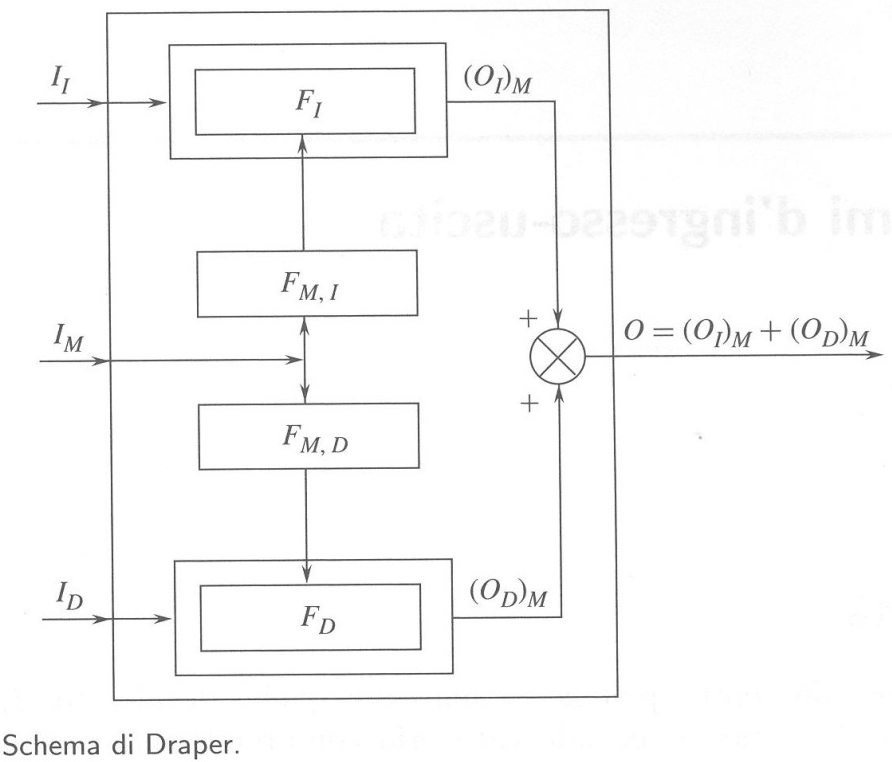
\includegraphics[width=0.5\linewidth]{fig/screenshot028}
		\label{fig:screenshot028}
	\end{figure}	
	In cui:
	\begin{itemize}
		\item[$\rightarrow$] $I_I$ è l'ingresso interferente, ovvero la grandezza di influenza.
		
		Ricordi il termometro a resistenza? Deformando il provino può variare la resistenza. 
		
		\item[$\rightarrow$] $I_M$ è l'ingresso modificante, ovvero quella variazione che può modificare la stessa funzione $F$.
		
		Magari per un fattore ambientale può variare la resistività $\rho$ nella formula della resistenza o la costante $K$ della molla di una bilancia. 
		
		\item[$\rightarrow$] $I_D$ è l'ingresso desiderato.
		
		\item[$\rightarrow$]  $F$ è la funzione di trasferimento tra input ed output, ad esempio nella molla, la funzione di trasferimento ideale, quella desiderata, è $F_D = 1/K$.		
	\end{itemize} 

	Nel seguente \underline{esempio} è mostrato come per un manometro ad U quale siano le possibili grandezze di influenza/interferenti.
	
	NB: una grandezza modificante cambierebbe proprio la NATURA del fluido.	
\begin{figure}[H]
	\centering
	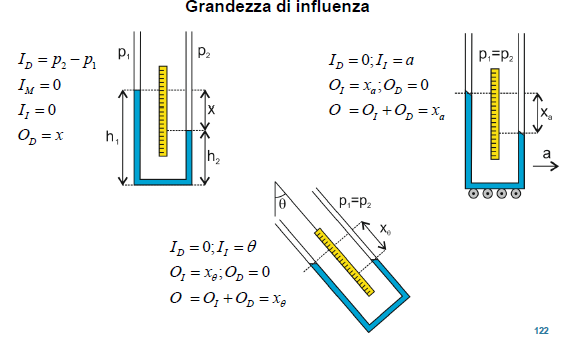
\includegraphics[width=0.7\linewidth]{fig/screenshot029}

	\label{fig:screenshot029}
\end{figure}
	È il costruttore di un trasduttore a dover specificare il campo di
	riferimento, l' intervallo di errore
	statico, ossia tutti quei valori in corrispondenza dei quali vengono garantiti i limiti
	definiti delle caratteristiche metrologiche dello strumento. \newline 
	
	Per limitare l'effetto delle grandezze d'influenza, queste possono essere: 
	\begin{itemize}
		\item \underline{Trascurate}  
		
		Il loro effetto, calcolato o stimato, non modifica in
		modo apprezzabile la misura:
		\[F_D = F_I \approx 0\]
		Si ignorano le grandezze di influenza, stando accorti all'incertezza finale di misura. \newline
		
		Lo schema di Draper non subisce modifiche.
		
		\item \underline{Corrette} 
		
		È noto l’effetto sul misurando e attraverso un calcolo si  corregge.
		
		Si stimano i contributi di $I_D, I_M$ e si sottraggono gli effetti sull'uscita. 		
\begin{figure}[H]
	\centering
	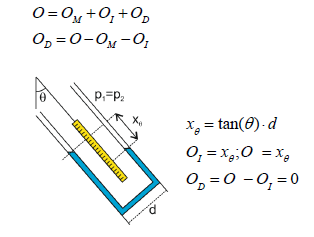
\includegraphics[width=0.5\linewidth]{fig/screenshot030}
	\label{fig:screenshot030}
\end{figure}
	
		\item \underline{Compensate} 
		
		Si adotta un dispositivo che generi un segnale opposto a quello
		generato dalla grandezza di influenza.
		
		Si aggiunge un ingresso che può essere modificante o interferente in grado di
		annullare l’effetto delle grandezze di influenza.
		
\begin{figure}[H]
	\centering
	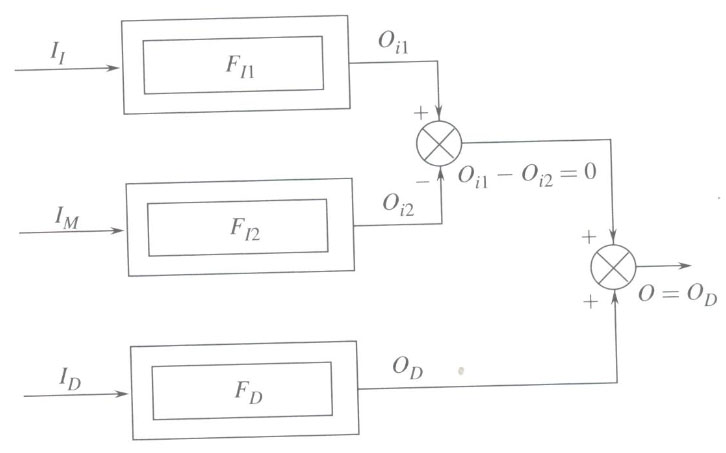
\includegraphics[width=0.5\linewidth]{fig/screenshot031}
	\label{fig:screenshot031}
\end{figure}

		Ad esempio, per un estensimetro, so che, se c'è $T$ come grandezza di influenza, allora si avrà come output:
		\[ R' = R_\varepsilon + R_T\]
		
		Traziono un provino e misuro così un $R = \dfrac{\Delta V}{I}$ non reale perché dipendente dalla grandezza d'influenza, nelle immediate vicinante pongo così un provino uguale, a cui è applicato lo stesso sensore, ma non lo trazioni, in questo modo, ipotizzando che il $\Delta T$ agisca su entrambi i provini allo stesso modo, ottengo un $R' = \dfrac{\Delta V'}{I'}$, ovvero un'uscita che compensa la grandezza interferente, sottraendo così quest'ultimo segnale, leggo automaticamente l'uscita corretta. 
		
		\item \underline{Eliminate} 
		
		Si fa in modo di controllarne le variazioni in modo da ridurre a livelli
		trascurabili gli effetti, rendo nullo l'effetto delle grandezze d'influenza, si eliminano a priori.
		
		Una metodologia di eliminazione si basa sull’applicazione di un filtro selettivo
		o soppressivo. \newline
		
		Un \textit{filtro soppressivo} è posto prima dell'input e sopprime, elimina i contributi delle grandezze interferenti e modificanti:		
\begin{figure}[H]
	\centering
	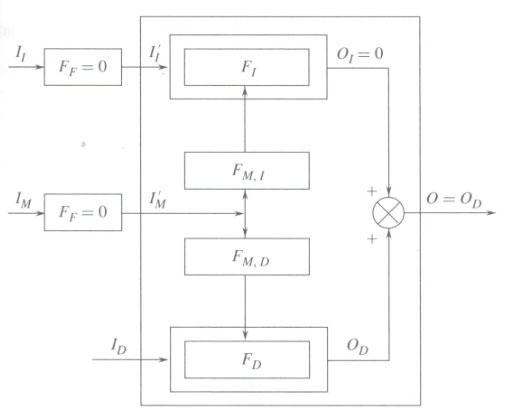
\includegraphics[width=0.5\linewidth]{fig/screenshot033}
	\label{fig:screenshot033}
\end{figure}
		Un \textit{filtro selettivo} è posto dopo l'output e sopprime, elimina l'effetto delle grandezze d'influenza o modificanti:		
\begin{figure}[H]
	\centering
	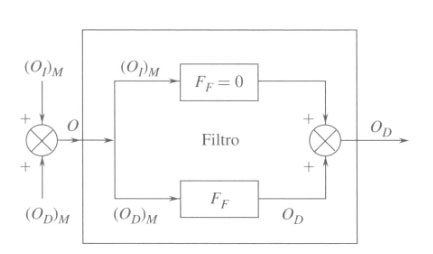
\includegraphics[width=0.5\linewidth]{fig/screenshot032}
	\label{fig:screenshot032}
\end{figure}


		\item \underline{Controreazione ad alto guadagno }
		
		Metodologia prediletta per strumenti di precisione, consiste nell'inserimento di un amplificatore ad alto guadagno limitando questo l'effetto delle grandezze interferenti. \newline 
		
		\underline{Esempio}: misuratore di tensione, galvanometro \newline 
		Cos'è un galvanometro? Il dispositivo è costituito da una bobina mobile solidale con una lancetta indicatrice sovrapposta ad una scala graduata, questa può parzialmente ruotare all'interno di un campo magnetico. Una molla tiene la bobina in posizione zero. Quando una corrente fluisce nelle spire, il solenoide genera un campo magnetico, che opponendosi a quello esterno produce una forza che fa ruotare la bobina e quindi l'ago indicatore. La molla contrasta la rotazione, con il risultato che l'angolo di deviazione è proporzionale all'intensità della corrente o tensione da misurare.
				
		In questo modo l'output sarà governato dalla funzione di trasferimento della molla e della bobina, in catena aperta:		
\begin{figure}[H]
	\centering
	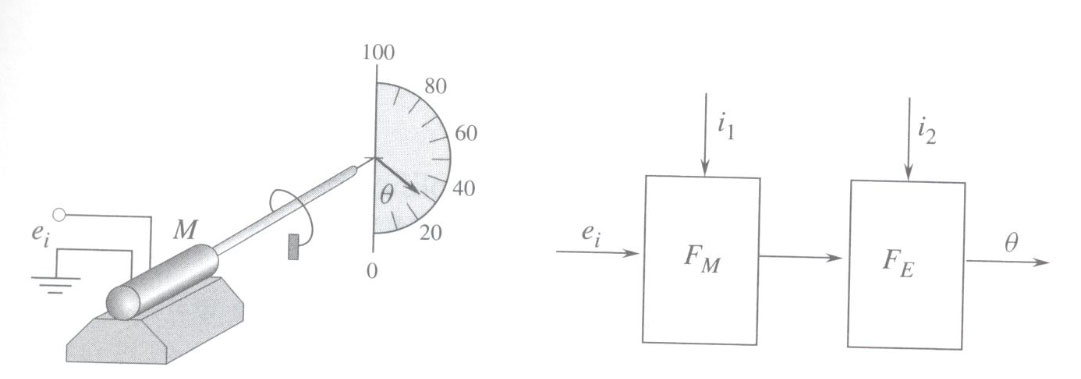
\includegraphics[width=0.5\linewidth]{fig/screenshot034}
	\label{fig:screenshot034}
\end{figure}
		\[ \vartheta = F_MF_E\cdot e_i\]
		
		Cosa succede si si applica un amplificatore ad alto guadagno e un potenziometro che fornisca un'uscita proporzionale alla rotazione dell'angolo? 
		
	La catena diventa chiusa:

\begin{figure}[H]
	\centering
	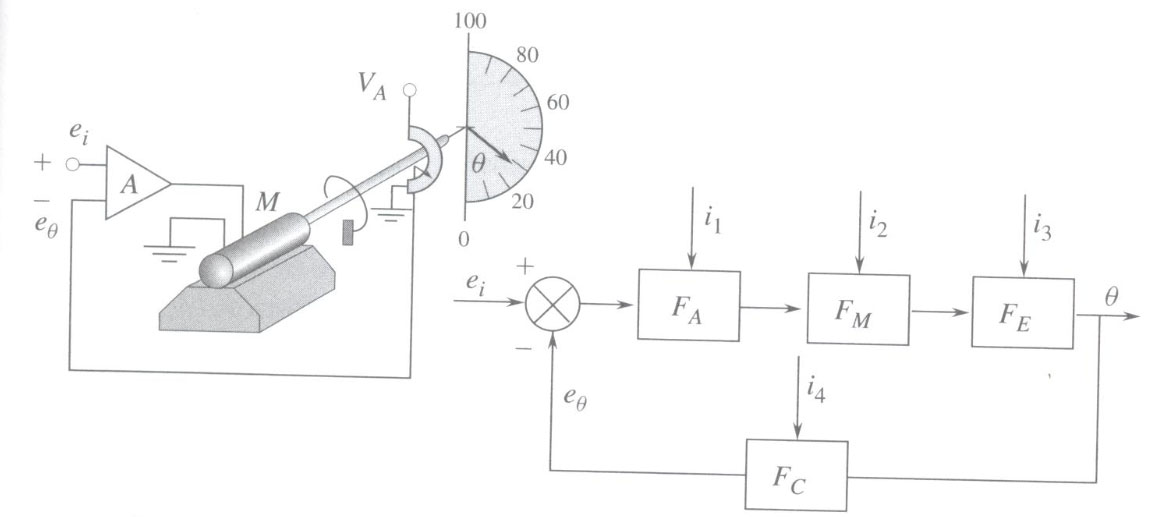
\includegraphics[width=0.5\linewidth]{fig/screenshot035}
	\label{fig:screenshot035}
\end{figure}

		\[\vartheta = F_AF_MF_E\cdot (e_i-e_\theta) \hspace{1cm} e_\theta = F_C\theta\]
		\[ \vartheta = \dfrac{F_AF_MF_E}{1 + F_AF_MF_EF_C}e_i\]
		Per un guadagno alto $F_A >>1$ si può trascurare il termine unitario ed effettuare le dovute semplificazioni:
		\[ \vartheta \approx \dfrac{1}{F_C}e_i\]
		Gli ingressi aggiunti non modificano l'output, che diviene soltanto funzione del potenziometro, semplificando non di poco la trattazione degli elementi interferenti e modificanti. 	
	\end{itemize}

\begin{figure}[H]
	\centering
	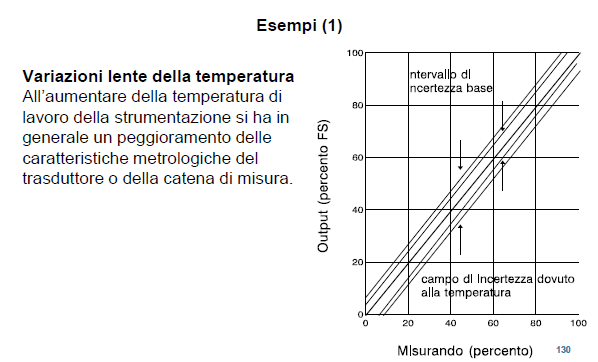
\includegraphics[width=0.7\linewidth]{fig/screenshot036}
	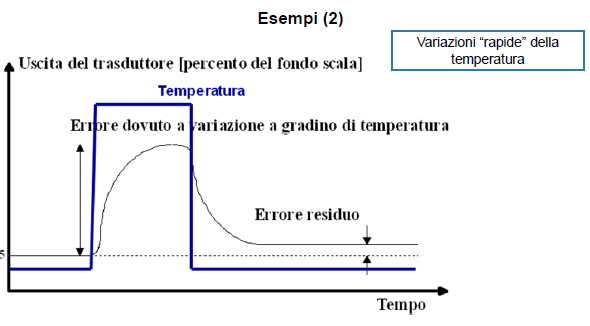
\includegraphics[width=0.7\linewidth]{fig/screenshot037}
	\label{fig:screenshot036}
\end{figure}
\begin{figure}[H]
	\centering
	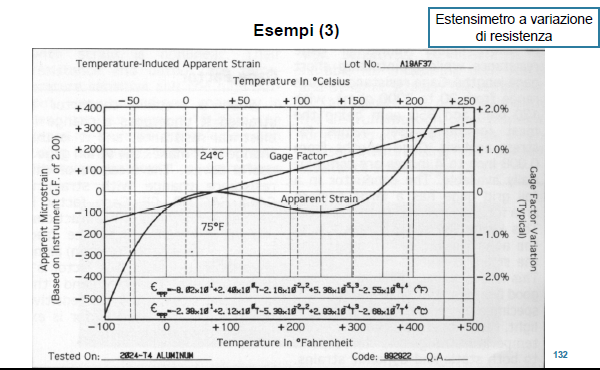
\includegraphics[width=0.7\linewidth]{fig/screenshot038}
	\caption{La deformazione apparente è solo dovuta ad un $\Delta T$, sapendo dal grafico che è di una certa entità, si può sottrarre o sommare per ricondursi al valore ininfluenzato.}
	\label{fig:screenshot038}
\end{figure}
\begin{figure}[H]
	\centering
	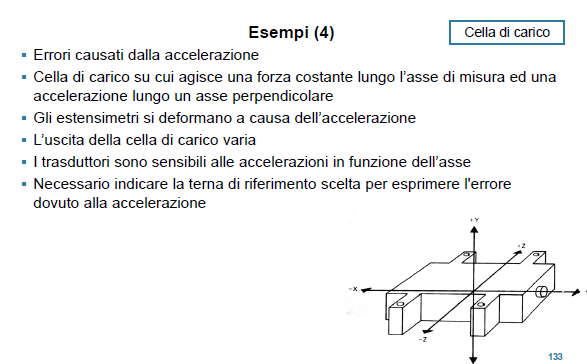
\includegraphics[width=0.7\linewidth]{fig/screenshot039}

	\label{fig:screenshot039}
\end{figure}
\begin{figure}[H]
	\centering
	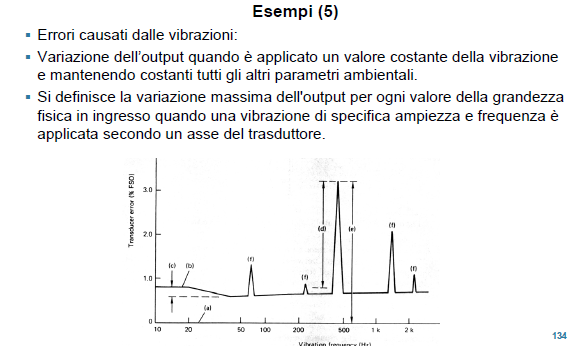
\includegraphics[width=0.7\linewidth]{fig/screenshot040}
	\label{fig:screenshot040}
\end{figure}

\begin{itemize}	
\item[$\Rightarrow$] \textbf{Campo di impiego per una grandezza d'influenza} 
 
		Campo entro il quale deve rimanere compresa una grandezza d'influenza
		durante la misurazione e/o la regolazione affinché sia possibile ottenere la
		misura del parametro.
		
		[UNI 4546, 3.5.1] 
		
\item[$\Rightarrow$] \textbf{Campo di sicurezza per una grandezza d'influenza} 
 
		Campo entro il quale deve rimanere compresa una grandezza d'influenza
		durante l'uso di un dispositivo per misurazione e/o regolazione affinché non
		risulti permanentemente alterata alcuna delle sue caratteristiche metrologiche.
		
		[UNI 4546, 3.5.2]
		
\item[$\Rightarrow$] \textbf{Campo di magazzino per una grandezza d'influenza} 


		Campo entro il quale deve rimanere compresa una grandezza d'influenza
		ambientale durante tutto il tempo in cui un dispositivo per misurazione e/o
		regolazione non è in funzione, affinché non risulti permanentemente alterata
		alcuna delle sue caratteristiche metrologiche: le grandezze d'influenza agiscono anche quando lo strumento non è in funzione! 		
\end{itemize}
		[UNI 4546, 3.5.3] \newline 
\end{adjustwidth}


\newpage
\section{Progettazione di una catena di misura}  
\begin{adjustwidth}{2in}{}

		Per progettare una catena di misura è necessario:
		\begin{enumerate}
			\item Identificare lo scopo per il quale la misurazione viene condotta,
			\item Fissare l'incertezza con la quale si vuol ottenere la misura;
			\item Progettare il processo di misurazione che implica sia la scelta hardware che
			delle procedure;
			\item identificare:
			\begin{enumerate}
				\item Il fenomeno da investigare;
				\item L’interazione tra il fenomeno ed il trasduttore;
				\item Il trasduttore;
				\item La restante parte della catena di misura;
				\item Il software;
				\item Il personale addetto alla misurazione;
				\item Le necessità di chi ha commissionato le misure;
				\item Gli utenti del prodotto;
			\end{enumerate}
		\end{enumerate} 
	Tenendo bene a mente che ognuna di questa fase è soggetta oltre che al rumore, anche da un'incertezza via via crescente.

\begin{figure}[H]
	\centering
	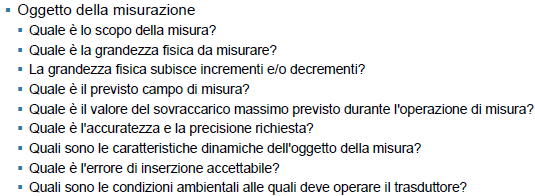
\includegraphics[width=0.5\linewidth]{fig/screenshot041}
	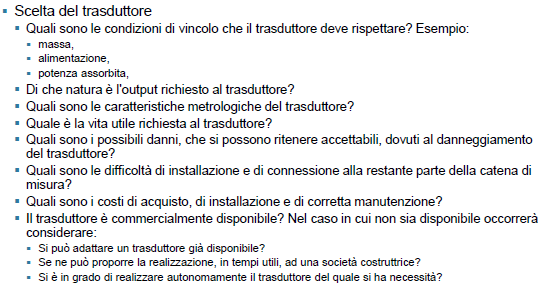
\includegraphics[width=0.5\linewidth]{fig/screenshot042}
	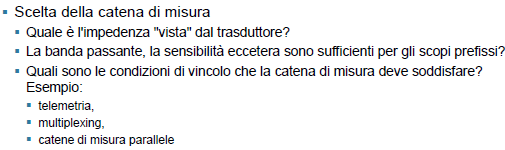
\includegraphics[width=0.5\linewidth]{fig/screenshot043}	
	\label{fig:screenshot041}
\end{figure}
\begin{figure}[H]
	\centering
	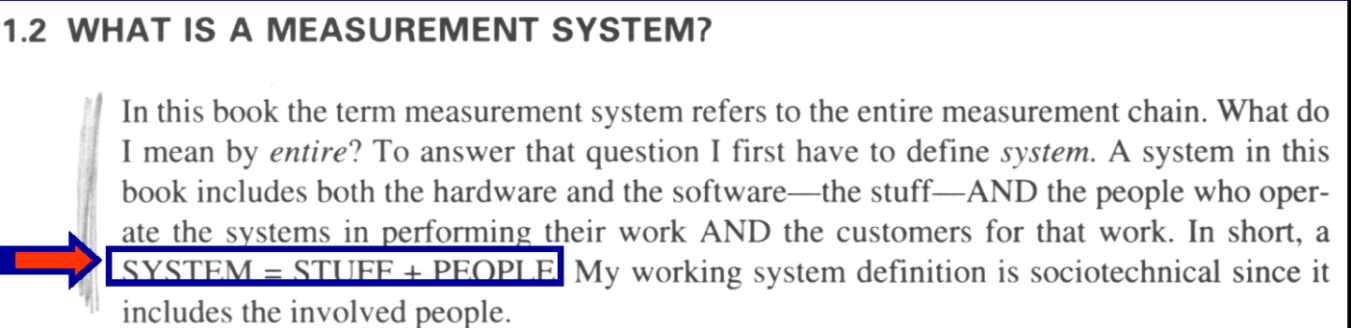
\includegraphics[width=0.7\linewidth]{fig/screenshot044}
	\label{fig:screenshot044}
\end{figure}

\end{adjustwidth}


\newpage
\section{Caratteristiche metrologiche dinamiche}  
\begin{adjustwidth}{2in}{}
	Con lo studio delle caratteristiche metrologiche dinamiche ci si chiede come varia l'uscita quando l'ingresso varia nel tempo. 
	\[y(t) = f(x(t))\]
	Questo porta alla costruzione di grafici in cui nelle ascisse sarà riporta il tempo mentre sulle ordinate saranno riportati sia l'ingresso $x$ che l'uscita $y$. \newline 
	
	Ci si pone sotto l'ipotesi di sensibilità unitaria, questo per evitare di moltiplicare l'uscita per un chicchessia valore, si suppone così per semplicità di visualizzate un'uscita omogenea e coincidente all'entrata. 
	
	Ad esempio per un termometro valeva $\Delta h = \dfrac{\alpha V}{A}\Delta T$, in questo caso se \newline $S = \dfrac{\alpha V}{A} = 1 \Rightarrow \Delta h = 1 \cdot \Delta T$. 
	
	È importante notare come questo sia un'idealizzazione: ricalcando il grafico in uscita quello d'entrata, falsa la realtà, in un caso reale questa idealizzazione non vale. 
	
 
\begin{figure}[H]
	\centering
	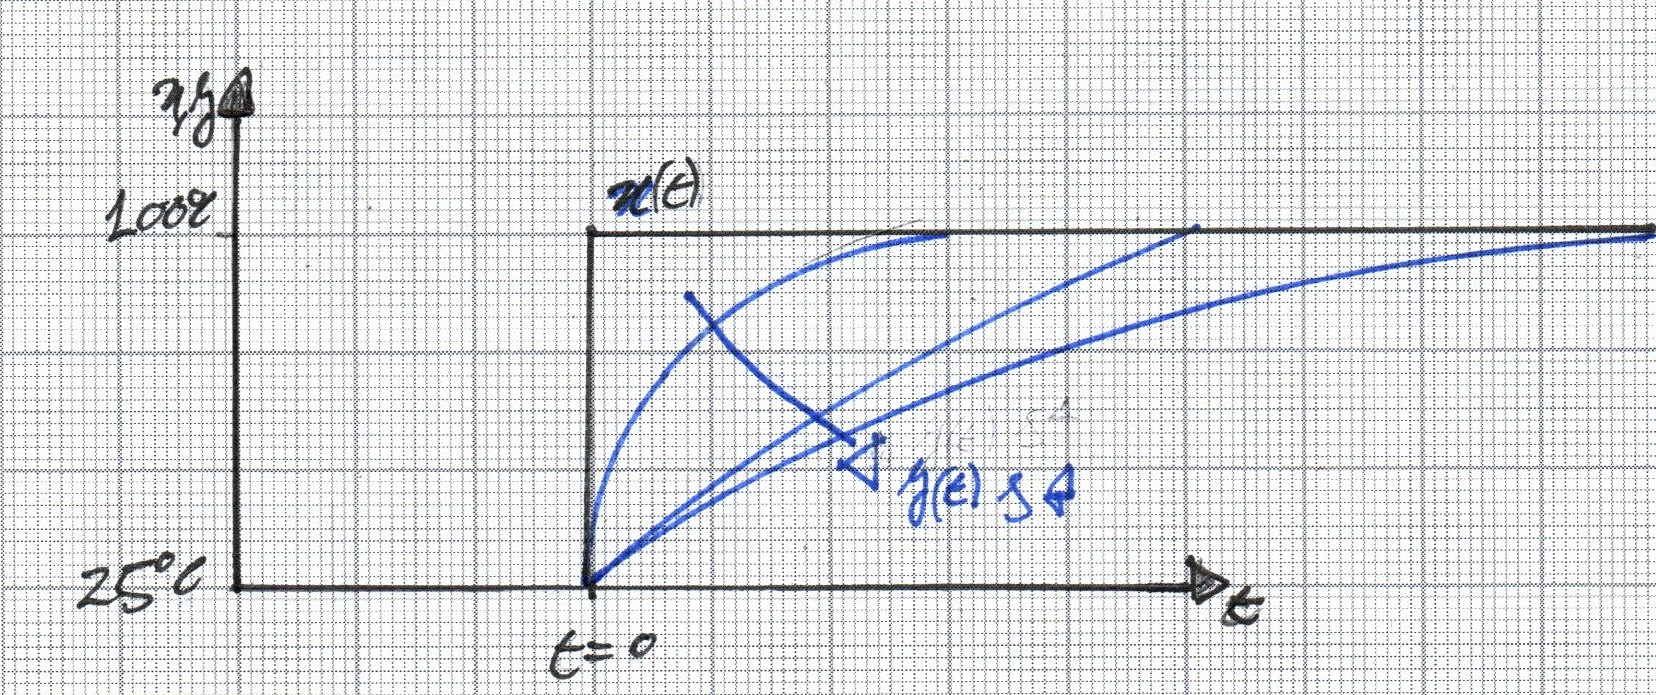
\includegraphics[width=0.5\linewidth]{fig/screenshot045}
	\label{fig:screenshot045}
\end{figure}

\begin{figure}[H]
	\centering
	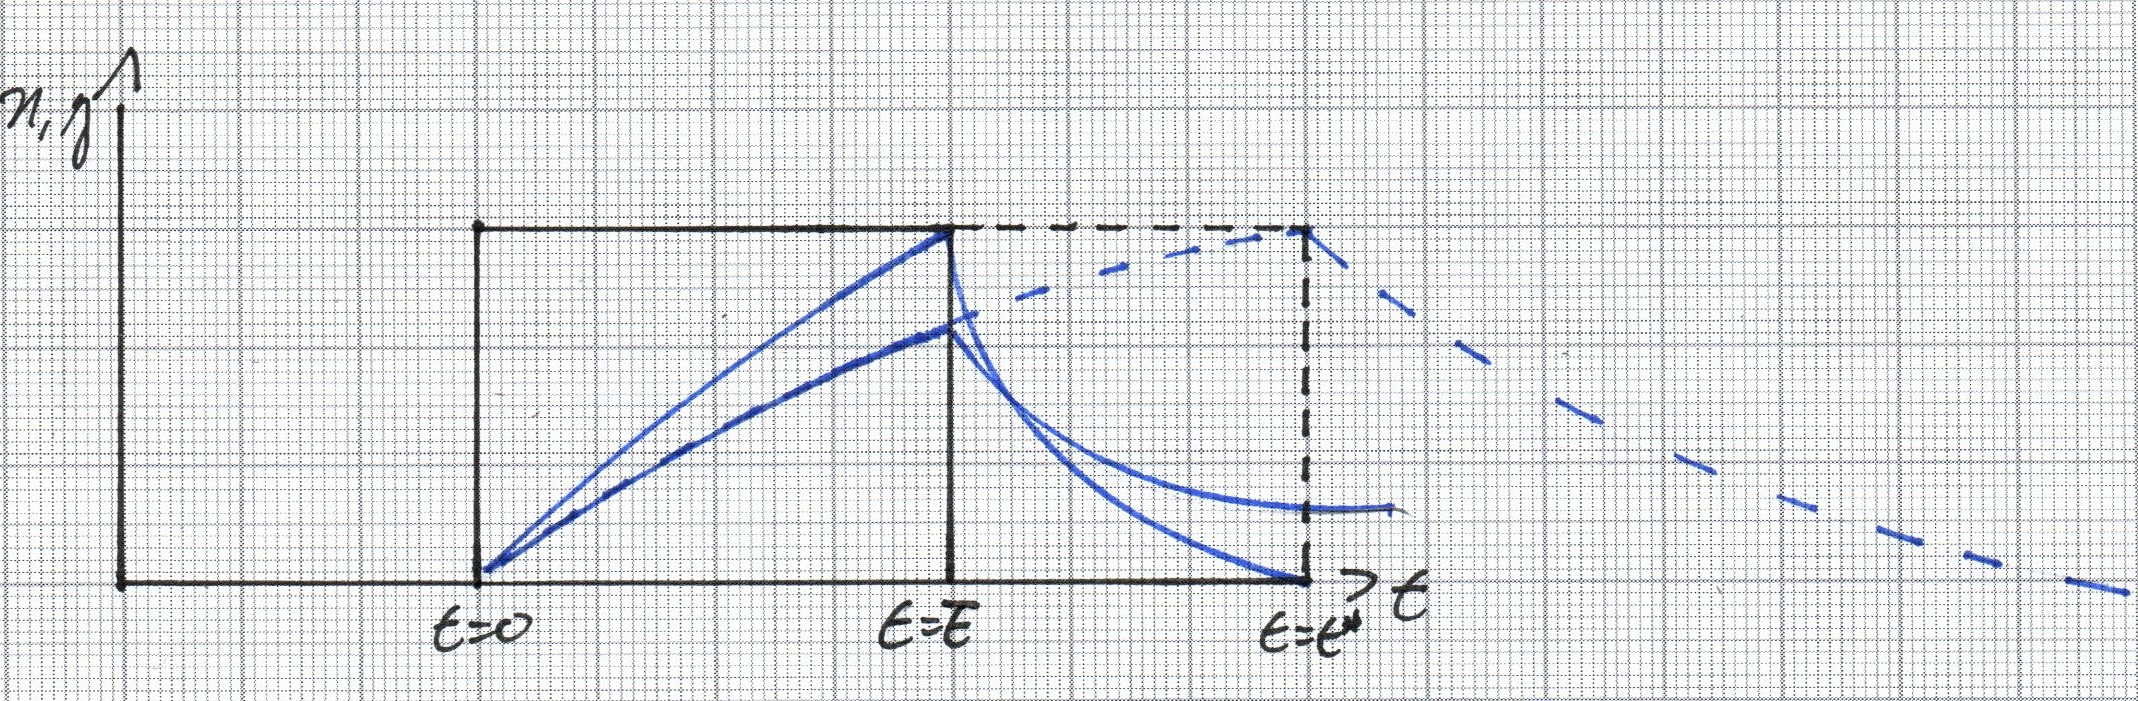
\includegraphics[width=0.5\linewidth]{fig/screenshot046}
	\label{fig:screenshot046}
\end{figure}

	Un segnale generico, com'è rappresentato? 
	
\begin{figure}[H]
	\centering
	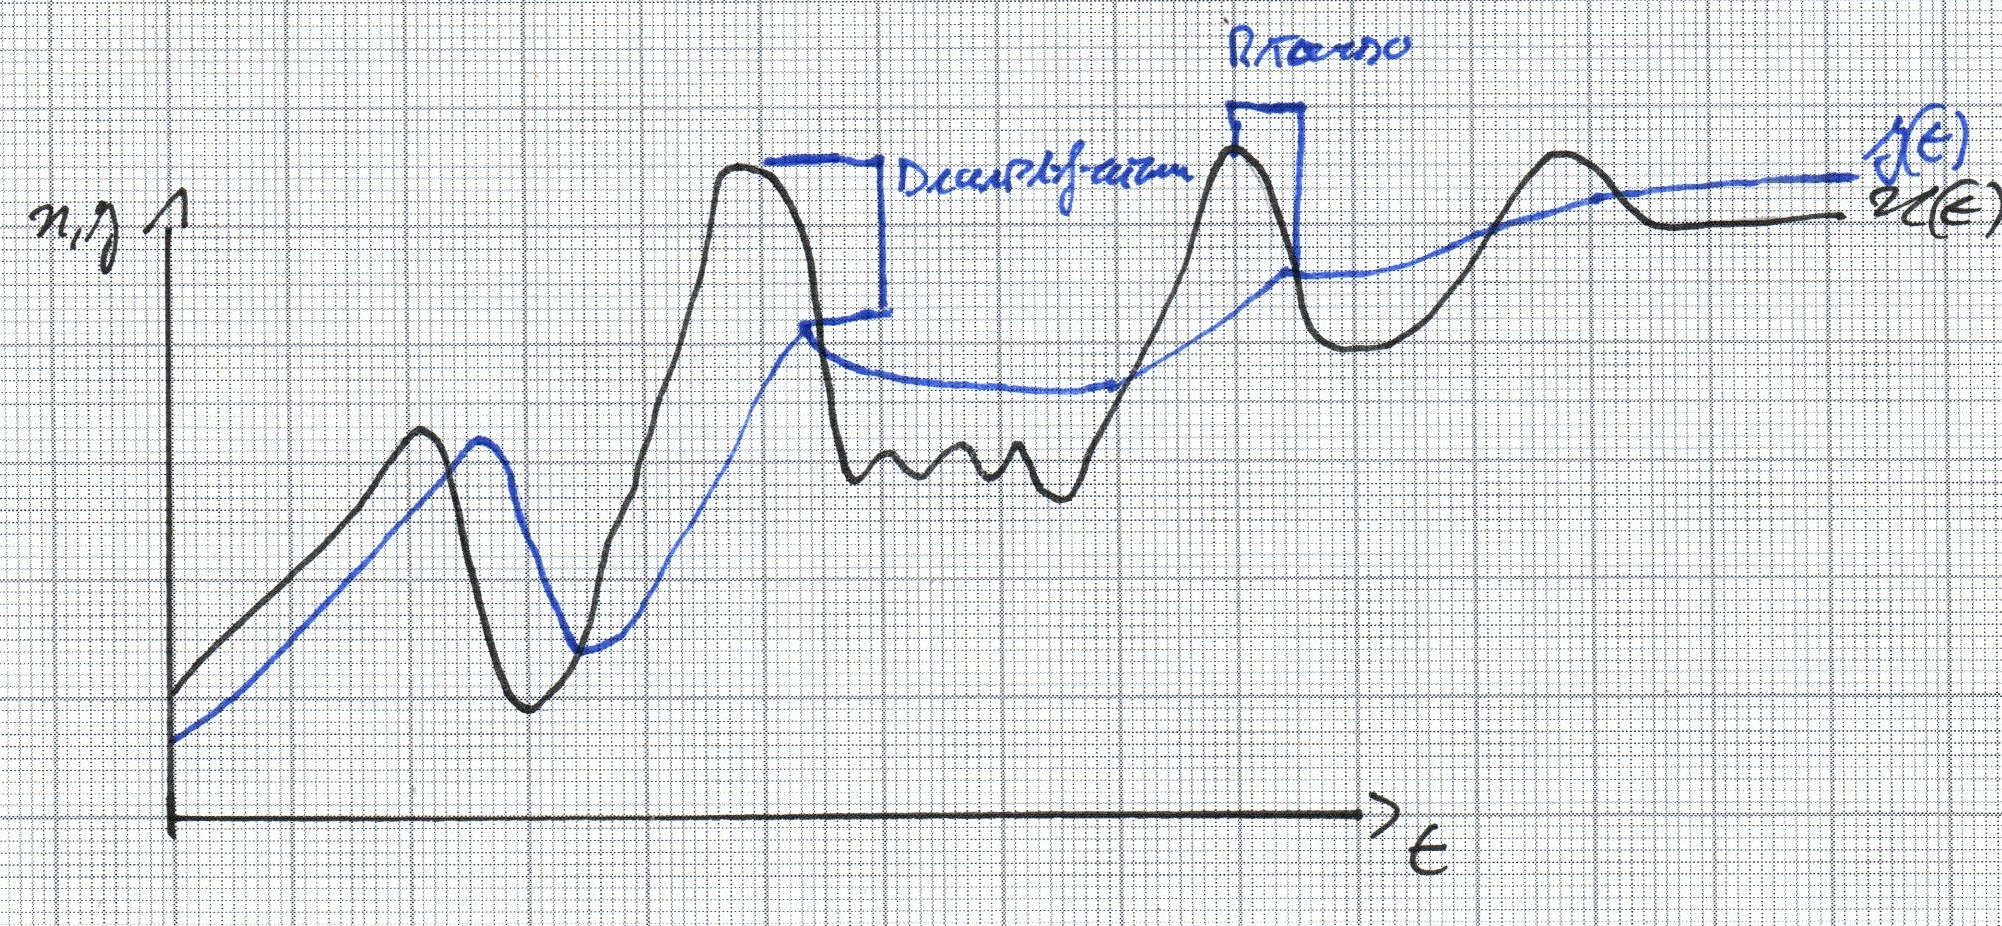
\includegraphics[width=0.5\linewidth]{fig/screenshot047}
	\label{fig:screenshot047}
\end{figure}

	Come risponde lo strumento al segnale? Si lavora fornendogli ingressi noti, in questo modo si potrà valutarne il comportamento dinamico. \newline 
\newpage	
	Si danno 3 tipi di ingresso: 
	\begin{enumerate}
		\item \textbf{Rapidamente variabile nel tempo} 
		 
		Rappresentato da una funzione d'ingresso a gradino crescente o decrescente. 
		
		Si possono dare anche input impulsivi, che corrisponderebbero a gradini crescenti e decrescenti molto ravvicinati. 
		
		\item \textbf{Lentamente variabile nel tempo} 
		 
		Rappresentato da un andamento a rampa.
		
		
		Nell'esempio precedente del termometro, un andamento a rampa può essere visualizzato se magari a $100 \degree C$ si spegne il fuoco e idealmente la temperatura ritorna "a rampa" all'equilibrio. 
		
		\item \textbf{Ingresso periodico} 
		 
		Un ingresso sinusoidale nel tempo. 
	\end{enumerate}

	\textbf{1. Ingresso rapidamente variabile nel tempo}  
\begin{figure}[H]
	\centering
	\includegraphics[width=0.5\linewidth]{fig/screenshot048}
	\label{fig:screenshot048}
\end{figure}
	\begin{itemize}
	\item \underline{Tempo morto dello strumento} $T_m$: tempo necessario per arrivare al $10\%$ del valore finale. 
	\item \underline{Tempo di salita} $T_s$: tempo necessario per arrivare dal $10\%$ al $90\%$ del valore finale.
	\item \underline{Tempo di rispost}a $T_r$: tempo necessario per arrivare dallo $0\%$ al $90\%$ del valore finale, somma dei precedenti tempi. 
	\item \underline{Sovra-elongazione}: massima distanza in ampiezza tra la prima sovra-elongazione ed il valore asintotico.
	\item \underline{Errore dinamico} $\pm \varepsilon_d$.
	
	Ad esempio, nel grafico è rappresentato un $\varepsilon_d=10\%$.
	\item \underline{Tempo di stabilizzazione} $T_st$: tempo necessario affinché l'uscita entri all'interno della banda di $\varepsilon_d$ e non esca più. 
	
	Ad esempio, se si aumenta la banda di $\varepsilon_d$, il tempo di stabilizzazione diminuisce, ma si lavora con uno strumento soggetto a maggior errore.
\end{itemize}
	\textbf{2. Ingresso lentamente variabile nel tempo} 
\begin{figure}[H]
	\centering
	\includegraphics[width=0.5\linewidth]{fig/screenshot049}
	\label{fig:screenshot049}
\end{figure}
	\begin{itemize}
	\item \underline{Tempo di ritardo} $T_r$: quantifica il fatto che l'uscita arriva alla stessa quota dell'ingresso in ritardo, la risposta partirà sempre un po' ritardata e continuerà a seguire il segnale d'ingresso parallelamente. 
	\end{itemize}
\newpage	
	\textbf{3. Ingresso periodico} \newline 
	Grazie alle serie di Fourier si può vedere un generico ingresso periodico come una somma di seni a diverse frequenze, una trasformata di Fourier si può addirittura applicare a qualsiasi tipo di segnale, anche pseudo-periodico. 
	
	Se viene dato un ingresso: 
	\[ x(t) = \sum_{i=1}^{n} x_{0i}\sin(2\pi f_i t)\]
	Come varia l'uscita? 
	\[ y(t) = \sum_{i=1}^{n} y_{0i}\sin(2\pi f_i t + \phi_i)\]
	Dove con $\phi_i$ identifico lo sfasamento. \newline 
	
	Un segnale caotico e generico si può così studiare considerando che effetto hanno le singole sinusoidi che lo compongono, per ogni uscita, per singola frequenza: valendo la sovrapposizione degli effetti è come se si studiasse lo strumento separatamente ad ogni frequenza analizzando cosa succede. \newline
	
	Si immagini di avere un segnale periodico così scomposto in frequenza:
	\[x(t) = 5\sin(2\pi t) + 2\sin(20\pi t) + 0.5\sin(100\pi t)  \]
	È un segnale composto da un segnale che oscilla tra $\pm 5$ alla frequenza di $1Hz$, un segnale che oscilla tra $\pm 2$ alla frequenza di $10Hz$ e di un segnale che oscilla tra $\pm 0.5$ alla frequenza di $50Hz$. \newline 
	
	Si supponga adesso misurare un segnale in uscita pari a: 
	\[y(t) = 3\sin\left(2\pi t + \dfrac{\pi}{8}\right) + 0.1\sin\left(20\pi t \dfrac{\pi}{16}\right) + \dots  \]
	Si noti innanzitutto come il segnale in uscita subisca chiaramente una deamplificazione, il primo passa dall'oscillare tra $\pm 5$  a $\pm 3$, mentre il secondo addirittura da $\pm 2$ a $\pm 0.1$. 
	
	E poi, in questo caso, valendo la sovrapposizione degli effetti, posso studiare lo strumento a $1Hz$, $10Hz$ e $50Hz$. \newline 
	
	Se la sinusoide è lenta, la frequenza è bassa, $y$ riesce a seguire il segnale, cosicché sia lo sfasamento che la deamplificazione risultino nulli.  	
\begin{figure}[H]
	\centering
	\includegraphics[width=0.5\linewidth]{fig/bassafreq}
	\label{fig:bassafreq}
\end{figure}

\newpage

	Se la sinusoide è più veloce, aumentando la frequenza, l'uscita riesce poco a seguire l'ingresso, si verifica che sia lo sfasamento che la deamplificazione sono non nulli. 	
\begin{figure}[H]
	\centering
	\includegraphics[width=0.3\linewidth]{fig/bassafreq1}
	\label{fig:bassafreq1}
\end{figure}

	Continuando ad aumentare la frequenza l'uscita fa sempre più fatica a stare dietro al segnale. 	
\begin{figure}[H]
	\centering
	\includegraphics[width=0.3\linewidth]{fig/bassafreq2}
	\label{fig:bassafreq2}
\end{figure}

	Al limite 	
\begin{figure}[H]
	\centering
	\includegraphics[width=0.3\linewidth]{fig/bassafreq3}
	\label{fig:bassafreq3}
\end{figure}


	Dov'è quindi che bisogna studiare i segnali? 
	
	Si introduce il guadagno come il rapporto tra il segnale in uscita e quello in ingresso: 
	\[ G_i = \dfrac{y_0}{x_0}\]
\newpage
	Ed il segnale può essere così studiato sul grafico guadagno-frequenza.
\begin{figure}[H]
	\centering
	\includegraphics[width=0.5\linewidth]{fig/nyquist1}
	\caption{Grafico guadagno-frequenza}
	\label{fig:nyquist1}
\end{figure}
	A $f=0$ si porrà avere segnale costante, mentre $G=1$ sarà null'altro che una condizione ideale, qualsiasi frequenza viene fornita, l'uscita riuscirà sempre ad inseguirla; la realtà dei fatti è però ben diversa: alle alte frequenze il guadagno diminuisce.  \newline 
	
	Un altro grafico su ohppen si possono studiare i segnali periodici è quello fase-frequenza, che risponde alla domanda, qual è lo sfasamento tra i segnali per ogni frequenza? 	

	Idealmente si vuole uno sfasamento nullo a tutte le frequenza, ma dato che è irrealizzabile una condizione del genere, ci si accontenterebbe  di avere una bisettrice, così magari alle basse frequenze lo sfasamento è basso e alle alte è alto, ricalcando magari il grafico del guadagno.
	\begin{figure}[H]
		\centering
		\includegraphics[width=0.3\linewidth]{fig/guad}
		\caption{Fase Irrealizzabile}
		\label{fig:guad}
	\end{figure}
	Il problema in questo caso è che il tempo di ritardo tenderebbe al limite all'infinito.
	
	E se si pone un tempo di ritardo sempre uguale per ogni frequenza? In questo caso, noto il valore $\phi_i = \omega_i t_r$ si potrebbe sottrarre e poi eliminare. \newline
	
	Quello che si nota invece sperimentalmente è che ch sarà sempre uno sfasamento di $ 180 \degree = - \pi$ con il seguente andamento. 
	
\begin{figure}[H]
	\centering
	\includegraphics[width=0.5\linewidth]{fig/nyquist2}
	\caption{Grafico fase-frequenza}
	\label{fig:nyquist2}
\end{figure}

	Quali parametri caratterizzano gli ingressi periodici? 
\begin{figure}[H]
	\centering
	\includegraphics[width=0.5\linewidth]{fig/mm1}
	\label{fig:mm1}
\end{figure}
	\begin{itemize}
	\item Frequenza di taglio $f_t$: frequenza alla quale si ha deamplificazione del guadagno pari a $3dB$. 
	\[ dB = 20 \log_{10}\left( \dfrac{G_f}{G_0}\right) \]
	\[ -3dB = 20 \log_{10}\left( \dfrac{G_{f_t}}{G_0}\right)  = 0.7 \]
	La frequenza di taglio si trova quando si raggiunge il $70\%$ del guadagno unitario.
	\item Banda passante dello strumento: tutte quelle frequenze per cui la deamplificazione è minore di $3dB$.
	\[[0;f_t]\]
	\end{itemize}
	Ad esempio, se tale banda fosse $[0;100]$ dando un input a $1Hz$ il guadagno è quasi unitario, mentre dando un input a $100Hz$ il guadagno è $0.7$, se come input dò un valore di 10, ritrovo un valore pari a 7, quindi con un errore del $30\%$.
	
	Questo ci dimostra che bisogna sempre stare lontano dal limite estremo della banda passante. \newline
	
	Per altre tipologie di strumenti la banda passante può essere 
	\[[f_{t1};f_{t2}]\]
\begin{figure}[H]
	\centering
	\includegraphics[width=0.5\linewidth]{fig/mm2}
	\label{fig:mm2}
\end{figure}
\newpage
	Per altri strumenti ancora può valere	
\begin{figure}[H]
	\centering
	\includegraphics[width=0.5\linewidth]{fig/mm3}
	\label{fig:mm3}
\end{figure}
	In questo caso la frequenza di taglio è definita come:
	\[3dB = 20 \log_{10}\left( \dfrac{G_{f_t}}{G_0}\right)  = 1.4\]
	Per cui la banda passante sarà quella per la quale non si arriverà ad amplificazione completa, sempre tra $ [0;f_t] $. 
\end{adjustwidth}

\newpage

\begin{adjustwidth}{2in}{}
	\textbf{{\LARGE NOTE}}
\end{adjustwidth}
	

\end{document}